\newpage
\chapter{Experiments and Results}
\label{chap:experiments}

This chapter reports four experiments aligned with the final presentation:
(1)~operationalizing maternal behavior in the training ecology,
(2)~testing plasticity and a Baldwin-style acceleration of adaptation,
(3)~measuring how initialization priors shape evolutionary trajectories, and
(4)~evaluating generalization on a held-out world$\times$food grid (E4 transfer).

\section{Common experimental setup}
\subsection{Environment and episode horizon}
Unless stated otherwise, each rollout uses a $15\times 15$ grid with one mother and one child, a configurable number of threat agents, and periodic food spawning. One episode lasts up to 1000 ticks.

\subsection{Food spawn interval (E4 grid)}
The parameter \textbf{food spawn interval} is the number of ticks between food spawns (with one food item per spawn in our runs).
A \textbf{shorter} interval means food appears more often:
interval~5 = \emph{abundant} food, interval~15 = \emph{medium} (training/emergence default), interval~25 = \emph{scarce} food.
In E4 figures, the food axis is labeled $5/15/25$ with $5$ on the abundant side and $25$ on the scarce side.

\subsection{Evolution and fitness}
Evolution follows the single-lineage $(1{+}1)$ scheme described in Chapter~3. Each evolutionary replicate is one mother lineage: a single heritable motivation-weight genome evolved over 3000 generations. Each candidate genome is evaluated over $N=10$ stochastic rollouts (different RNG seeds) and accepted only if mean fitness improves. Mutation uses $\epsilon\sim\mathcal{N}(0,0.05)$ applied elementwise to motivation weights (clamped to $[0.05,1.0]$).

Fitness uses Equation~\eqref{eq:fitness} with default $\alpha=0.5$ (child-weight) and $\lambda=0.002$ (injury penalty).

\subsection{Initialization regimes and plasticity regimes}
We compare three initialization regimes for motivation weights:
\texttt{anti\_maternal} (low Care/Protect, high Forage/Self),
\texttt{random\_uniform},
and \texttt{pro\_maternal} (high Care/Protect).
We also compare three adaptive regimes:
\textbf{E2} (evolution-only, no within-episode weight updates),
\textbf{P1} (outcome-based plasticity with an \emph{adaptive} learning rate scaled by deficit size, global deficit signal, per-tick updates), and
\textbf{P2} (outcome-based plasticity with a \emph{fixed} learning rate, local deficit signal, per-tick updates).

\subsection{Reported metrics}
Across experiments we report: normalized child/mother TTD, mother/child state trajectories (alive-tick means), conditional action probabilities $P(\text{Forage}\mid\text{hungry})$, $P(\text{Care}\mid\text{cold})$, $P(\text{Protect}\mid\text{injured})$, genome weight summaries, and child death-cause mixtures (hunger/cold/injury/alive).
Unless noted, emergence analyses use 30 independent evolution seeds; post-evolution evaluation uses 10 rollouts per final genome.

% =============================================================================
\section{Experiment 1: What ``maternal behavior'' looks like}
\subsection{Goal and training condition}
This experiment operationalizes ``maternal behavior'' as coordinated need-dependent switching between foraging, caregiving, and protection that improves child survival time (TTD) while maintaining maternal viability. The training condition uses a normal world with one threat and a medium food spawn interval (15 ticks between spawns), matching the final presentation.

\subsection{Survival across baseline conditions}
Figures~\ref{fig:exp1_ttd_boxplots} and~\ref{fig:exp1_km_child_mother} compare survival endpoints and full survival curves across baseline rollout conditions in that training ecology.
Child TTD varies substantially across conditions: some policies keep the child alive much longer (higher median and wider upper quartile on the boxplots), while others fail early.
Mother TTD shows a parallel spread, indicating that better child outcomes are not free---conditions that protect the child longer can still differ in how long the mother remains viable.
Kaplan--Meier curves make the timing explicit: conditions whose child curves decay more slowly sustain survival probability over more of the episode; mother curves show whether maternal death precedes or follows child failure.

\begin{figure}[H]
    \centering
    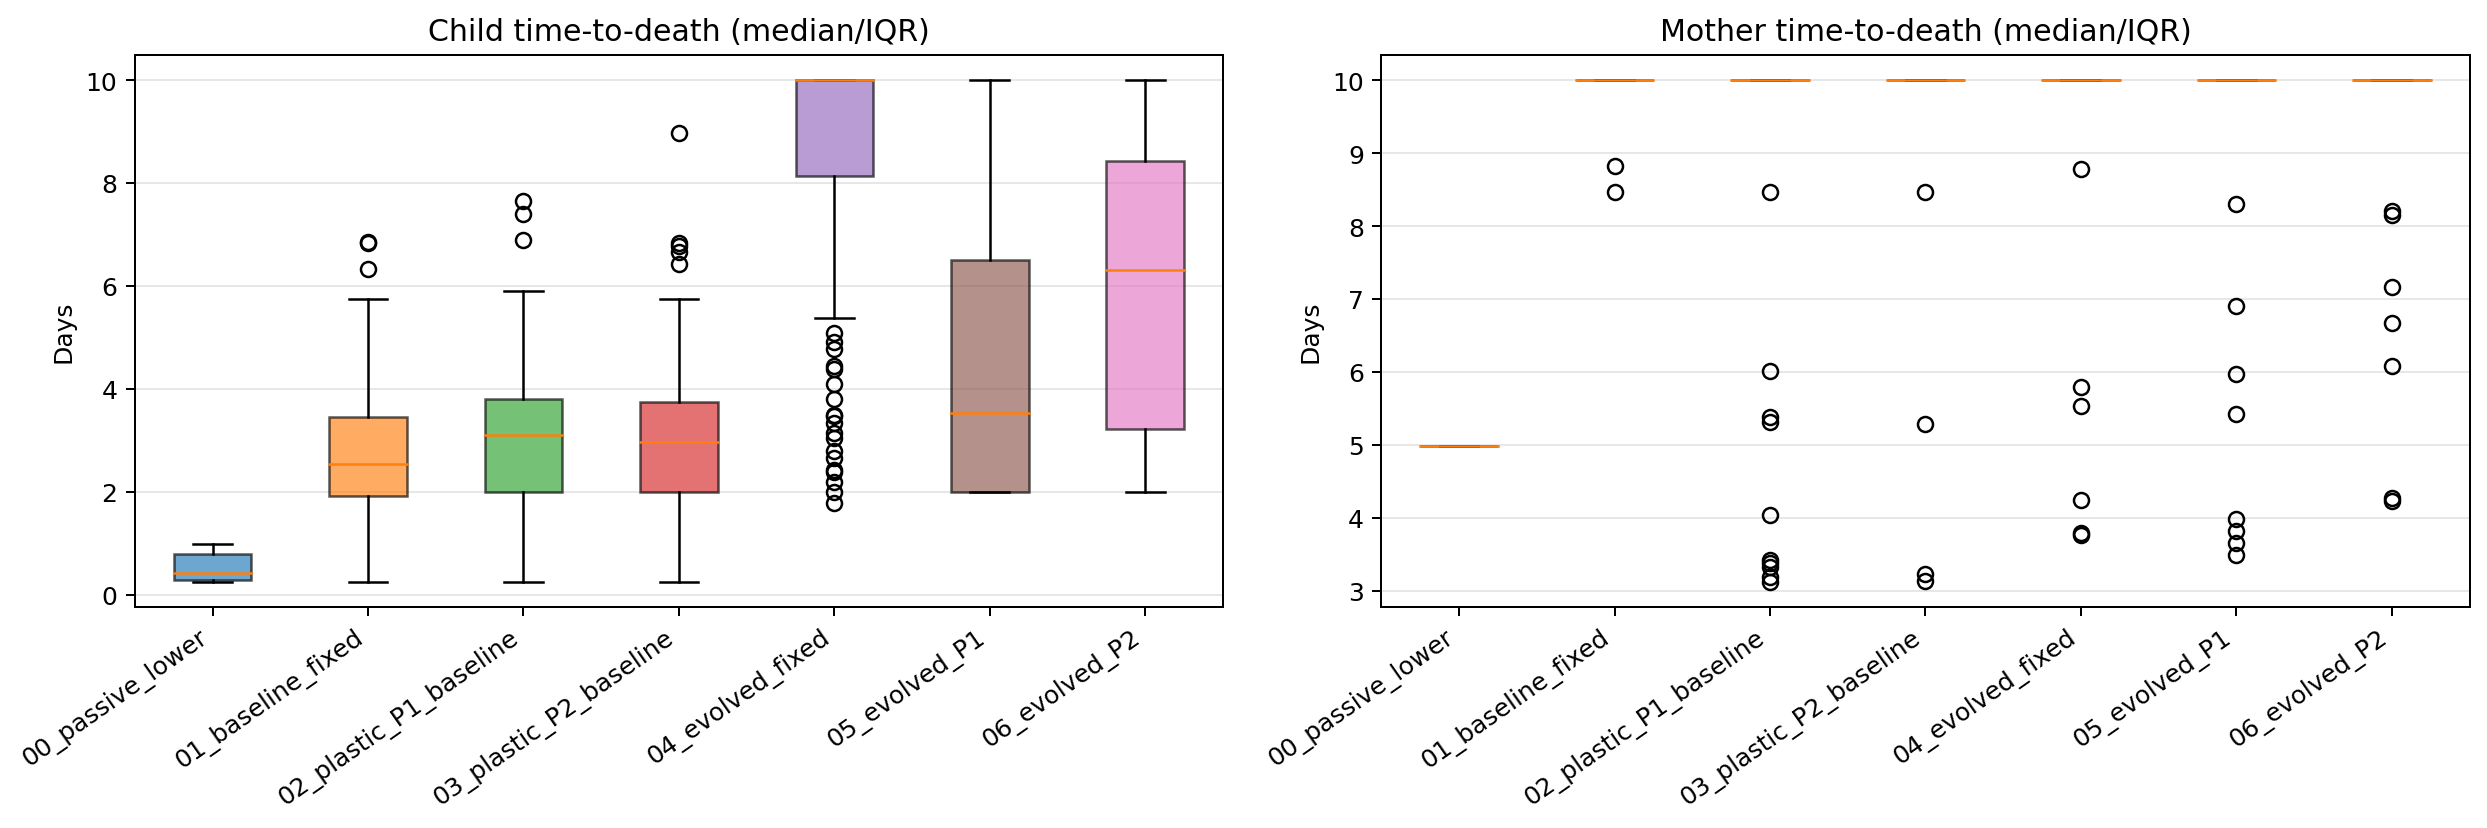
\includegraphics[width=0.9\linewidth]{plots/exp_1_plot_ttd_boxplots.png}
    \caption{Distribution of child (left) and mother (right) time-to-death across baseline rollout conditions in the training world. Boxes show median and interquartile range (IQR) over independent episode replicates. The y-axis is survival time in days (100 simulation ticks per day).}
    \label{fig:exp1_ttd_boxplots}
\end{figure}

\begin{figure}[H]
    \centering
    \begin{minipage}{0.49\linewidth}
      \centering
      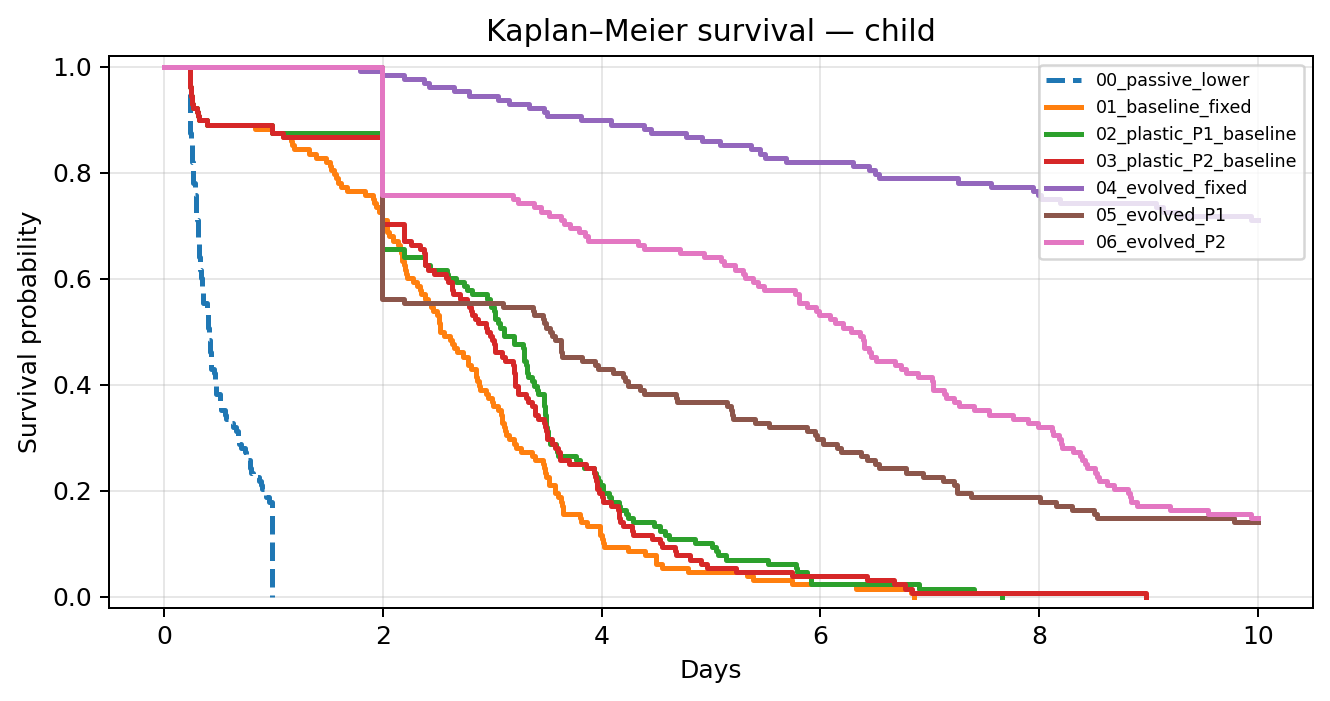
\includegraphics[width=\linewidth]{plots/exp_1_plot_km_child.png}
    \end{minipage}\hfill
    \begin{minipage}{0.49\linewidth}
      \centering
      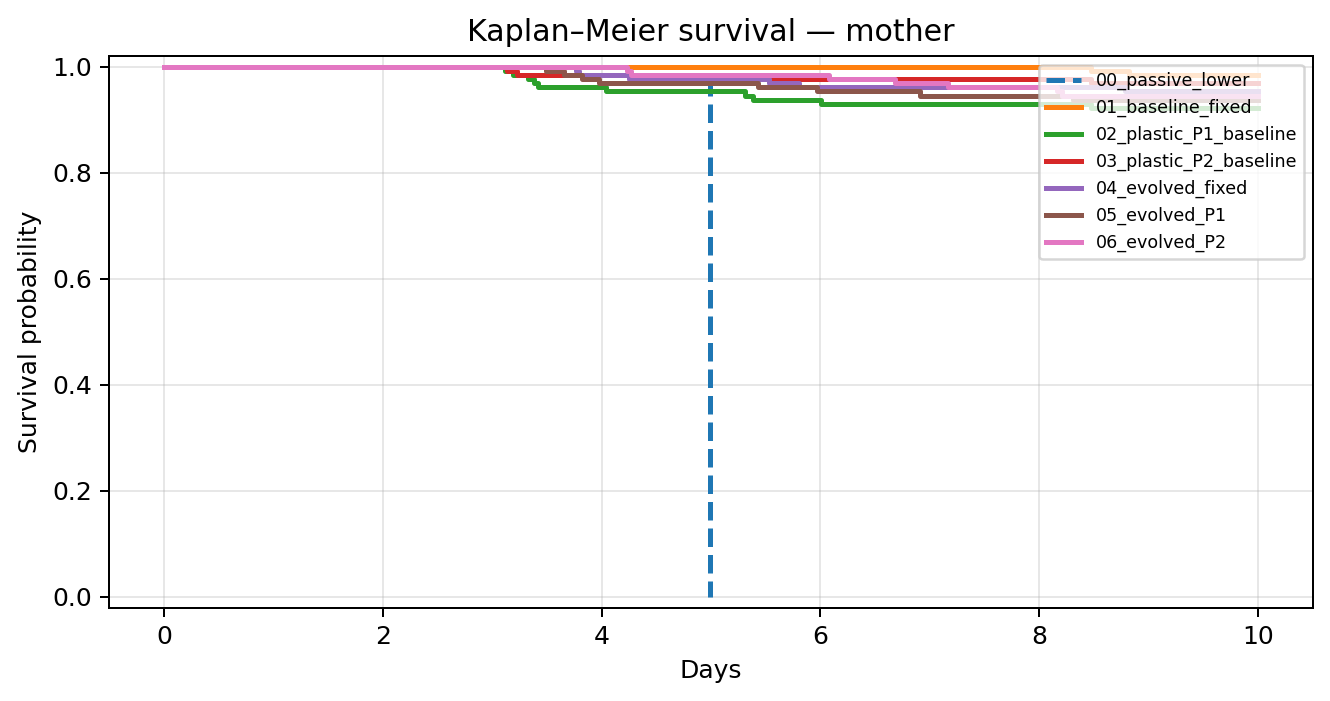
\includegraphics[width=\linewidth]{plots/exp_1_plot_km_mother.png}
    \end{minipage}
    \caption{Kaplan--Meier survival curves for child (left) and mother (right) by baseline condition.}
    \label{fig:exp1_km_child_mother}
\end{figure}

\subsection{Episode dynamics}
Figure~\ref{fig:exp1_internal_states} summarizes typical episode dynamics over 128 stochastic rollouts (mean $\pm$ std).
Panel~(a): mother and child can remain co-alive for a substantial fraction of the horizon when the policy is effective.
Panel~(b): child hunger, warmth, and injury on alive ticks---effective care keeps these in safer ranges while the child lives.
Panel~(c): Forage, Care, Self, and Protect are all used at non-negligible rates (motivational competition, not a frozen policy).
Panel~(d): mother energy, fatigue, bonding, \texttt{fear\_threat}, stress, \texttt{closeness\_child}, and slow endocrine traces (OT/CORT).

\begin{figure}[H]
    \centering
    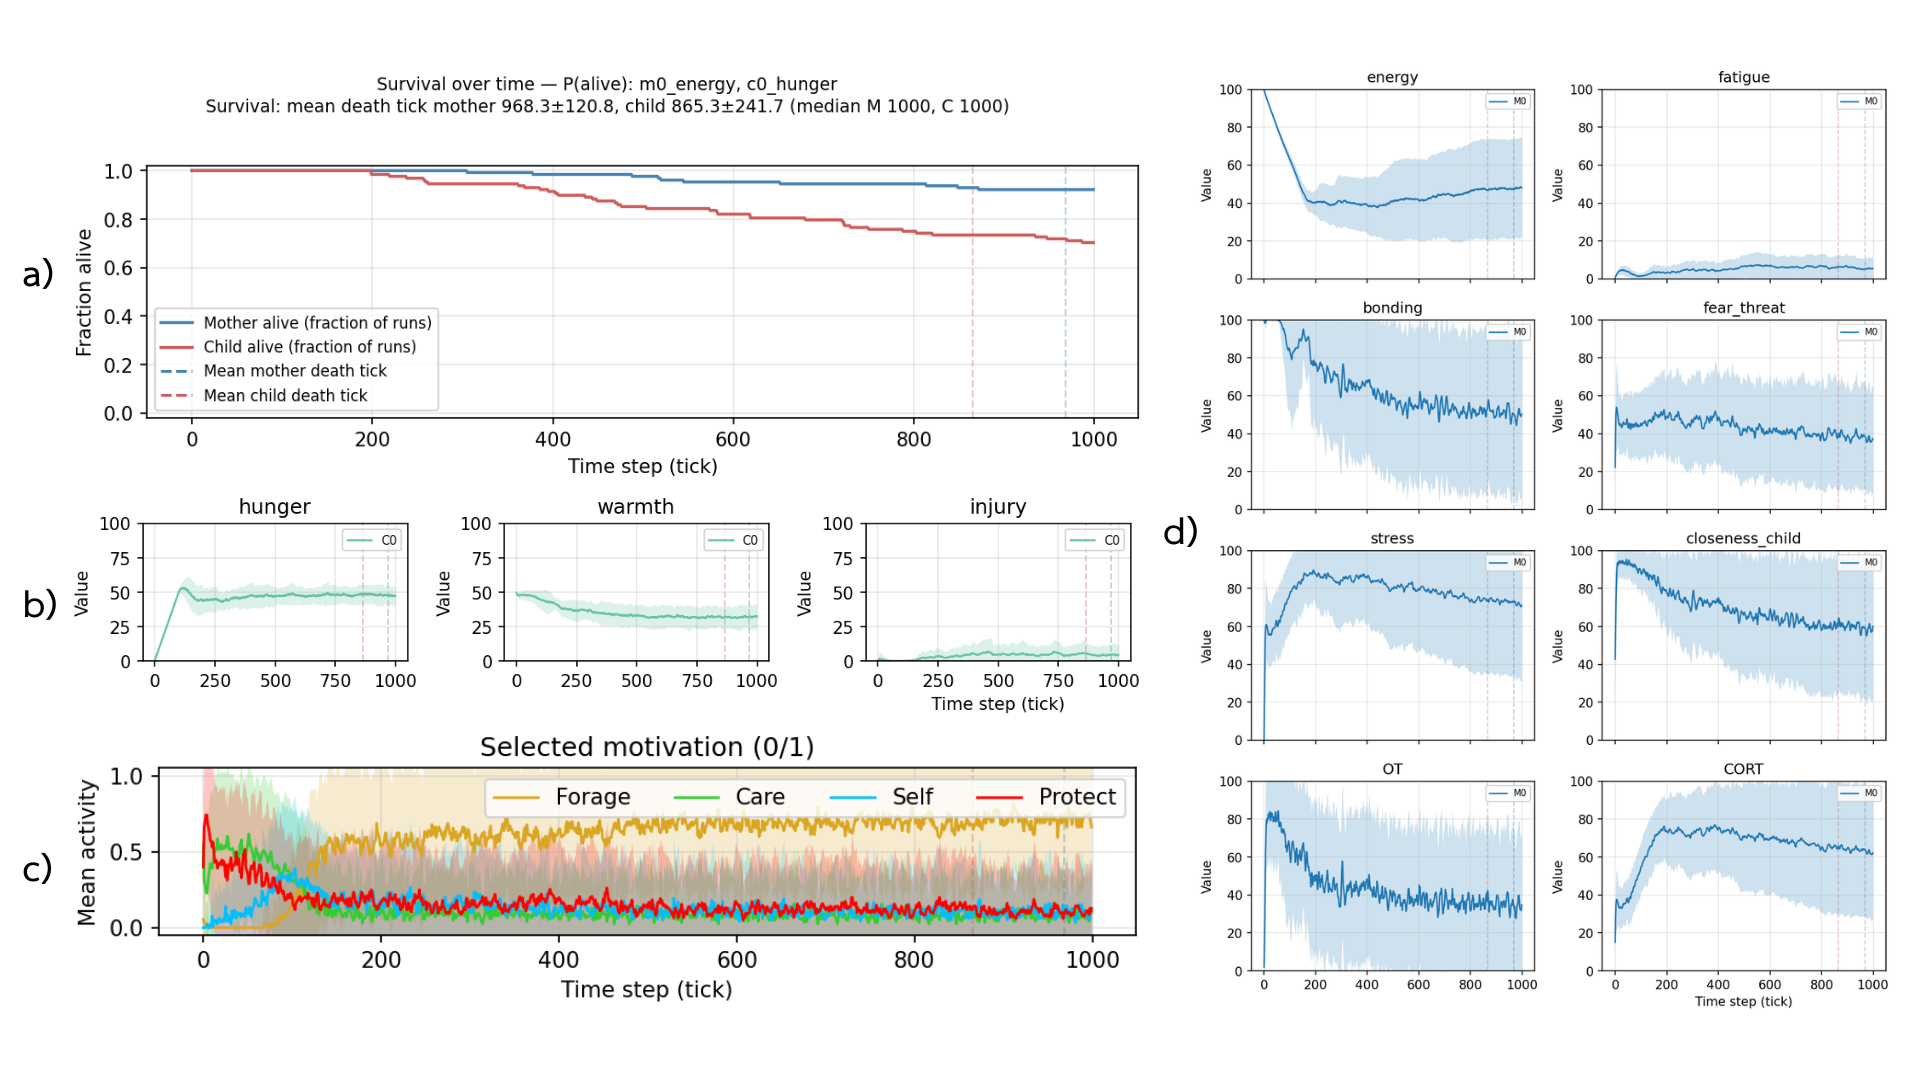
\includegraphics[width=\linewidth, trim={0 50 0 0}, clip]
    {plots/exp_1_internal_states.png}
    \caption{Representative rollout dynamics aggregated over 128 stochastic episode seeds (mean $\pm$ std): (a)~$P(\text{alive})$; (b)~child hunger, warmth, injury; (c)~motivation activity; (d)~mother internal states.}
    \label{fig:exp1_internal_states}
\end{figure}

\subsection{Takeaway (Experiment 1)}
The training world supports non-trivial mother--child dynamics: survival outcomes separate across conditions, and successful rollouts exhibit coordinated physiology, internal states, and motivation usage.

% =============================================================================
\section{Experiment 2: Role of plasticity and the Baldwin effect}
\subsection{Hypothesis}
Following the Baldwin effect, within-lifetime plasticity can improve behavior during an episode and can accelerate evolutionary adaptation even if learned changes are not inherited.

\subsection{Results}
Figure~\ref{fig:exp2_fitness_generations} sweeps world difficulty (easy, normal, hard) and child-fitness emphasis $\alpha_{\text{child}}\in\{0.3,0.5,0.7\}$, comparing E2, P1, and P2.
In virtually every panel, plastic runs (P1 red, P2 green) rise to higher fitness earlier than E2 (blue), with the gap most visible in normal and hard worlds.
The dashed traces (mean within-episode $|\Delta u_{\text{plastic}}|$) are largest in early generations and then flatten while fitness continues to improve---consistent with plasticity helping search early and inherited weights accounting for late performance.
The center panel (normal world, $\alpha=0.5$) matches the emergence setting used in Experiments~3--4.

\begin{figure}[H]
    \centering
    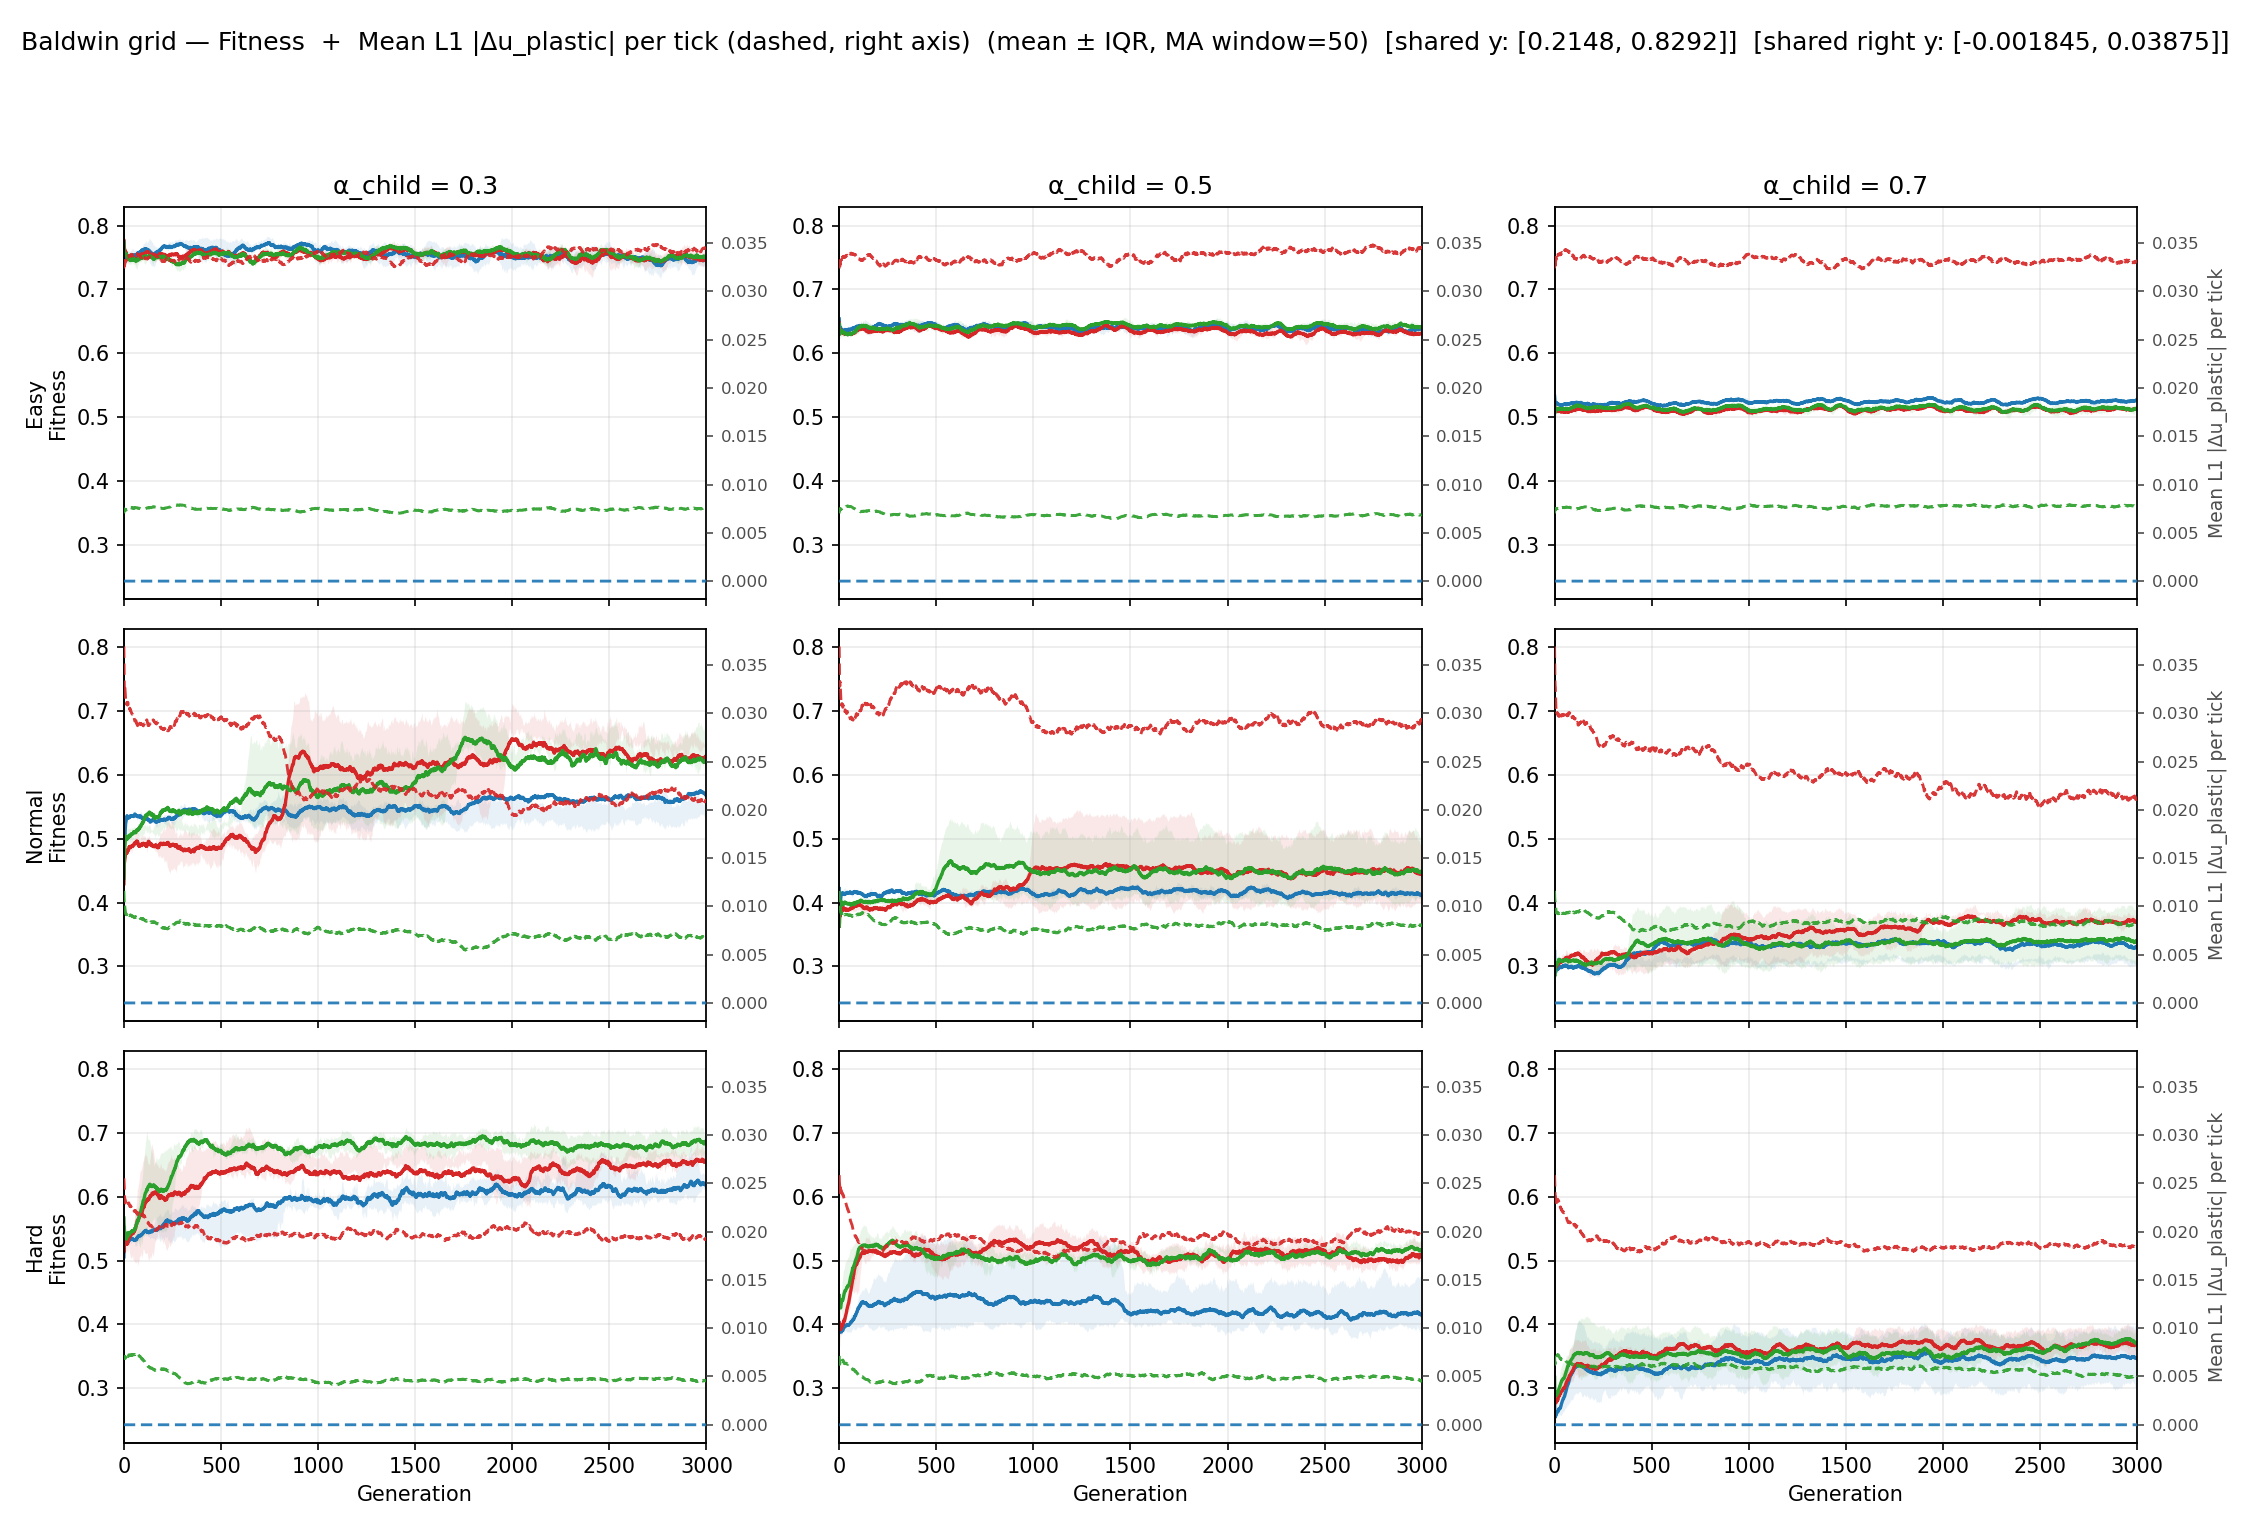
\includegraphics[width=\linewidth, trim={0 10 0 0}, clip]
    {plots/exp_2_baldwin_grid_fitness_du_plastic_allcond.png}
    \caption[Plasticity sweep (world $\times$ $\alpha_{\text{child}}$)]{Plasticity sweep: rows = world (easy/normal/hard); columns = $\alpha_{\text{child}}$ (0.3/0.5/0.7). Solid lines: mean fitness (E2 blue, P1 red, P2 green; IQR bands). Dashed: mean $|\Delta u_{\text{plastic}}|$ (right axis). Center panel = emergence training setting.}
    \label{fig:exp2_fitness_generations}
\end{figure}

\subsection{Takeaway (Experiment 2)}
Outcome-based plasticity (P1/P2) speeds evolutionary improvement relative to E2, especially under harder ecological pressure, motivating their inclusion in Experiments~3--4.

% =============================================================================
\section{Experiment 3: Effect of initial maternal traits}
\subsection{Hypothesis}
Initialization priors shape evolutionary trajectories: anti-maternal agents should shift most, random agents moderately, and pro-maternal agents least.

\subsection{Genome drift ($L_2$ over 30 lineages)}
Figure~\ref{fig:exp3_lineage_weights_l2} plots $L_2\|u(g)-u(0)\|$ during emergence (training world; mean $\pm$ SEM over 30 seeds).
Anti-maternal lineages (solid) reach the highest drift for all plasticities; pro-maternal (dotted) the least; random-uniform (dashed) in between---stable ordering anti $>$ random $>$ pro across E2, P1, and P2.

\begin{figure}[H]
    \centering
    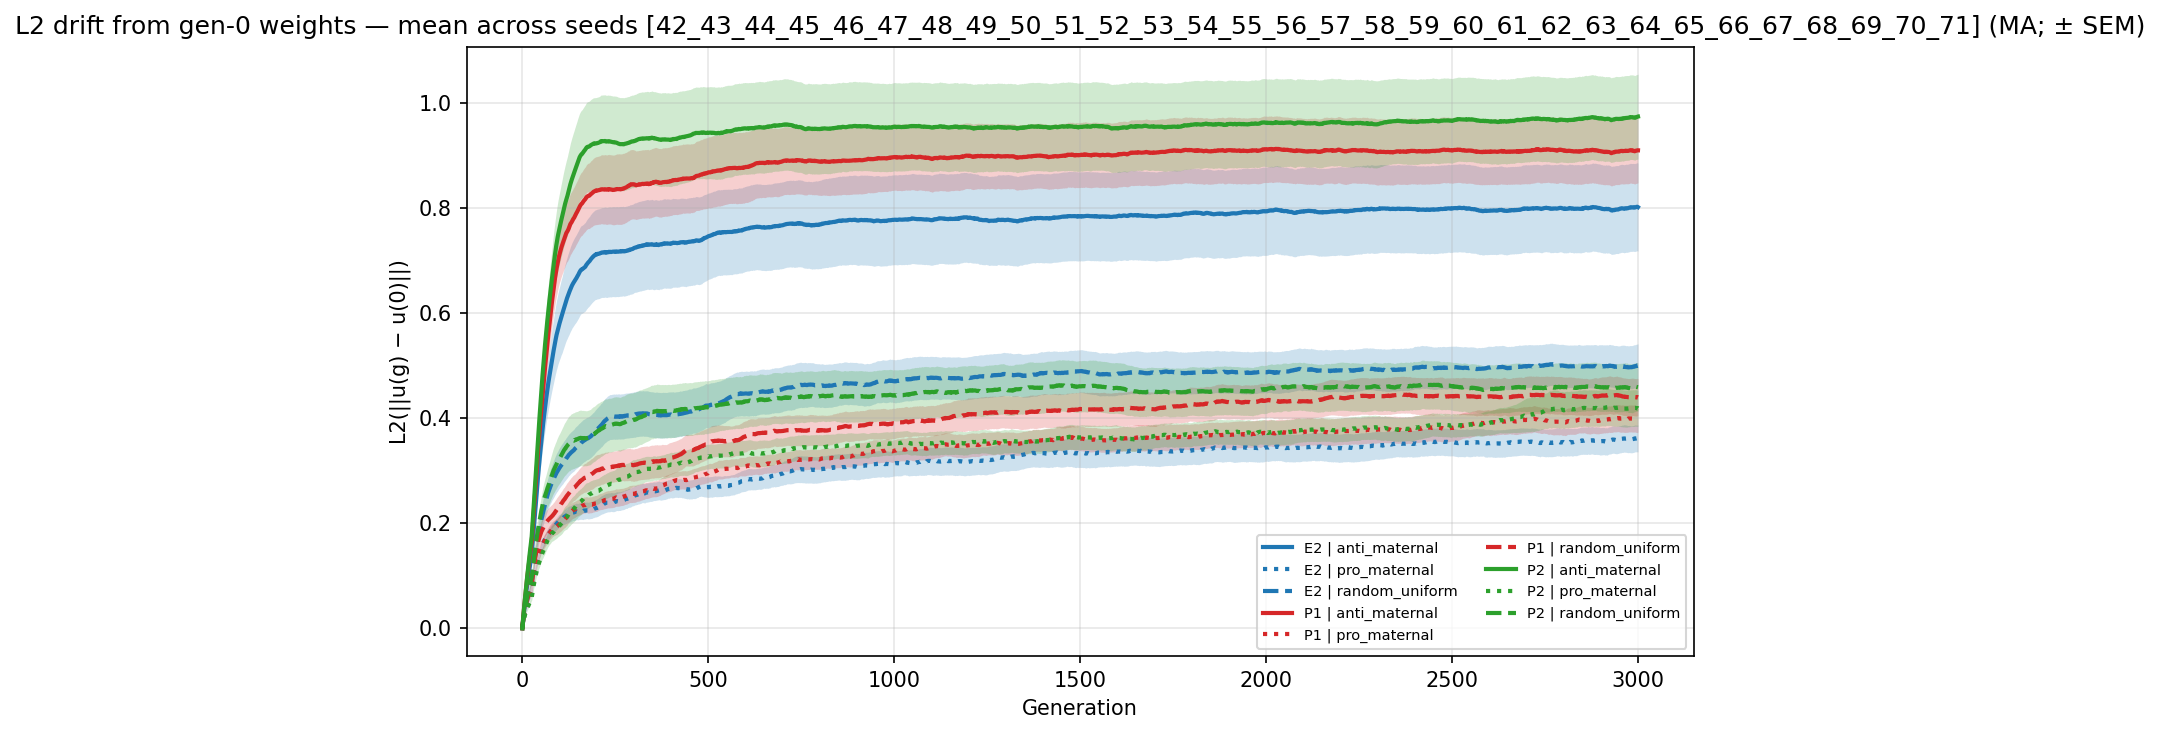
\includegraphics[width=\linewidth]{plots/exp_3_lineage_weights_l2_aggregate_ma_w50.png}
    \caption{$L_2$ genome drift vs.\ generation (MA window 50; mean $\pm$ SEM over 30 lineages). Color = plasticity; linestyle = initialization. Population aggregate, not one mother.}
    \label{fig:exp3_lineage_weights_l2}
\end{figure}

\subsection{Exemplar weight paths (one seed per init)}
Figure~\ref{fig:exp3_weight_transition} shows checkpoint heatmaps for \textbf{one} mother lineage per initialization (single $(1{+}1)$ run each), not averaged over seeds.
Anti-maternal runs reorganize Care/Protect leaves from low to high within the first 500--1000 generations; pro-maternal runs start near maternal profiles and change little; random runs adjust more diffusely.

\begin{figure}[H]
    \centering
    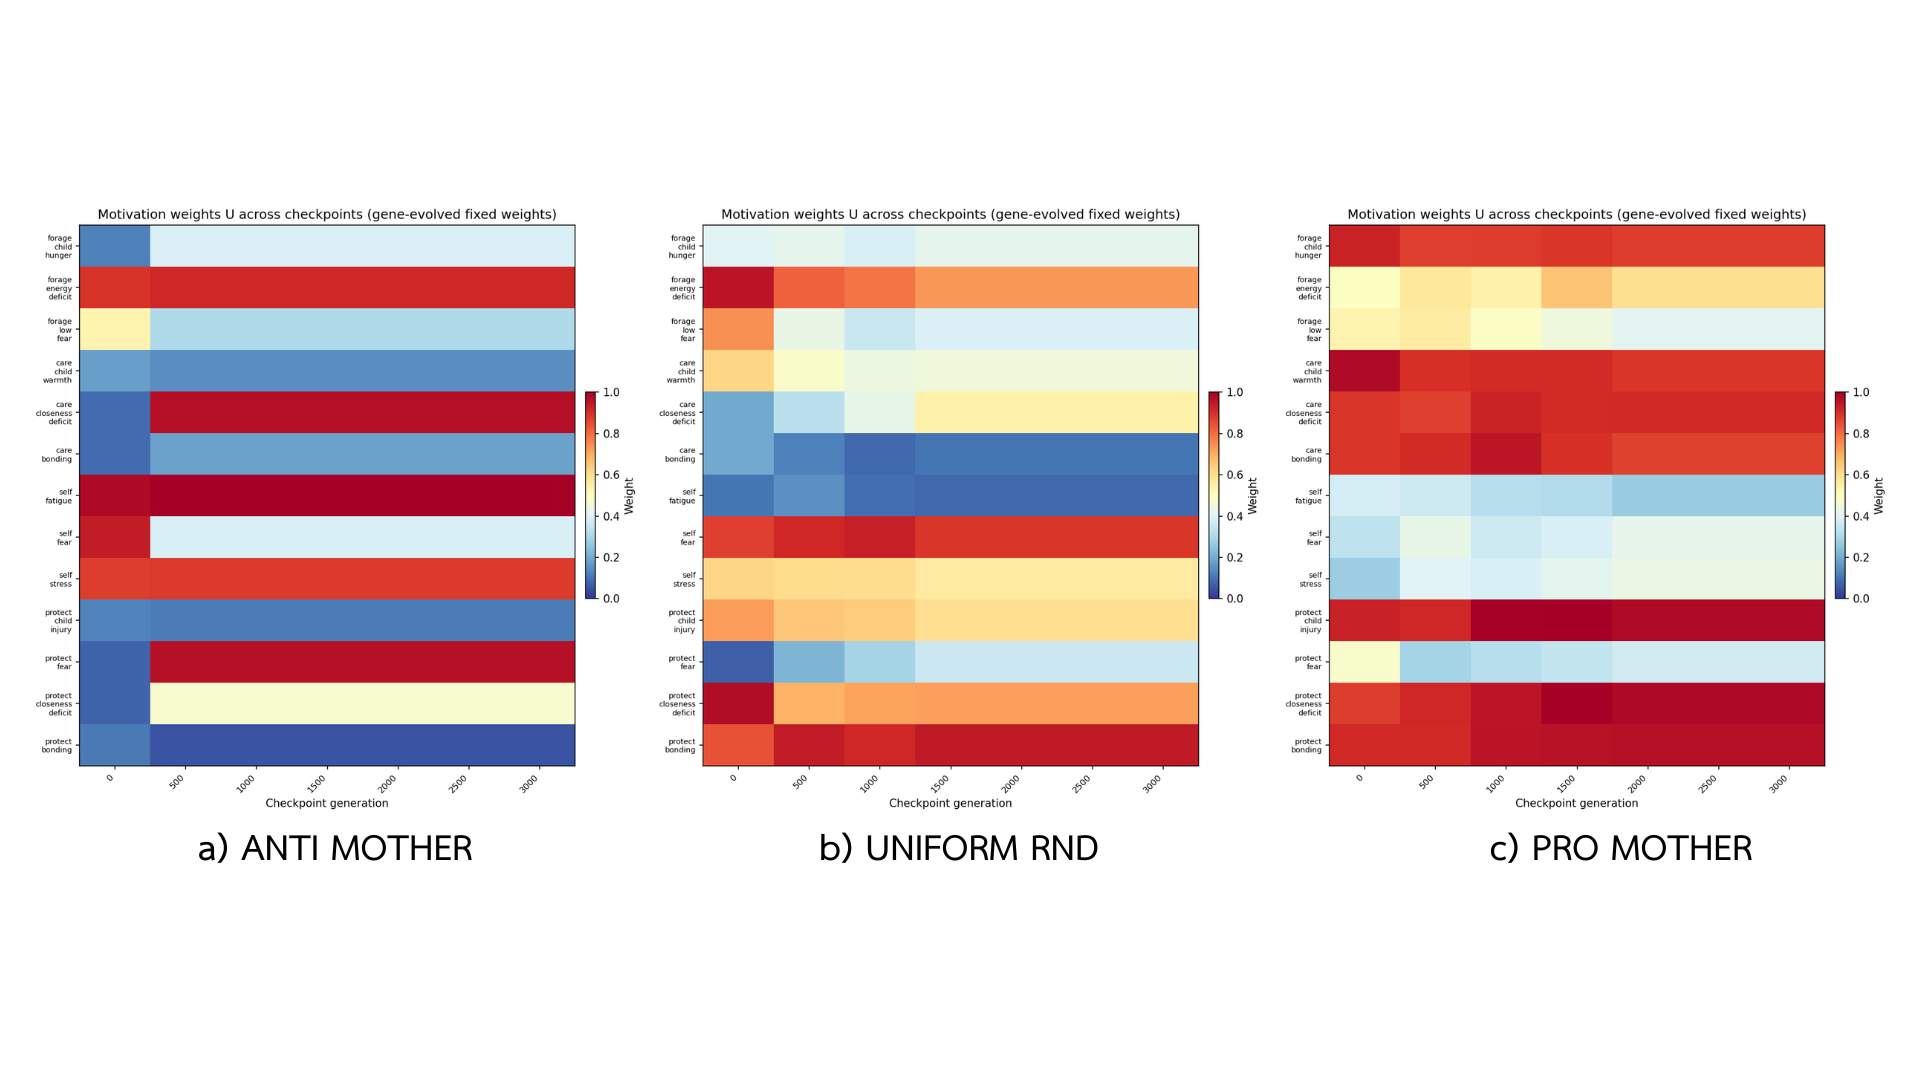
\includegraphics[width=\linewidth, trim={0 150 0 150}, clip]
    {plots/exp_3_weight_transition.png}
    \caption{Exemplar fixed-genome weights $u_{\text{fixed}}$ at checkpoints (0--3000, every 500 gens): one seed per init (anti / random / pro). Rows = 13 motivation leaves. Not a 30-seed average; see Figure~\ref{fig:exp3_lineage_weights_l2} for population drift.}
    \label{fig:exp3_weight_transition}
\end{figure}

\subsection{Per-weight and final init contrast (30 seeds)}
Figure~\ref{fig:exp3_weights} shows selected leaves by init$\times$plasticity cell (mean $\pm$ IQR over 30 lineages).
Figure~\ref{fig:exp3_diff_weights} shows final pro-minus-anti weight differences: partial convergence, with residual init signatures on several leaves.

\begin{figure}[H]
    \centering
    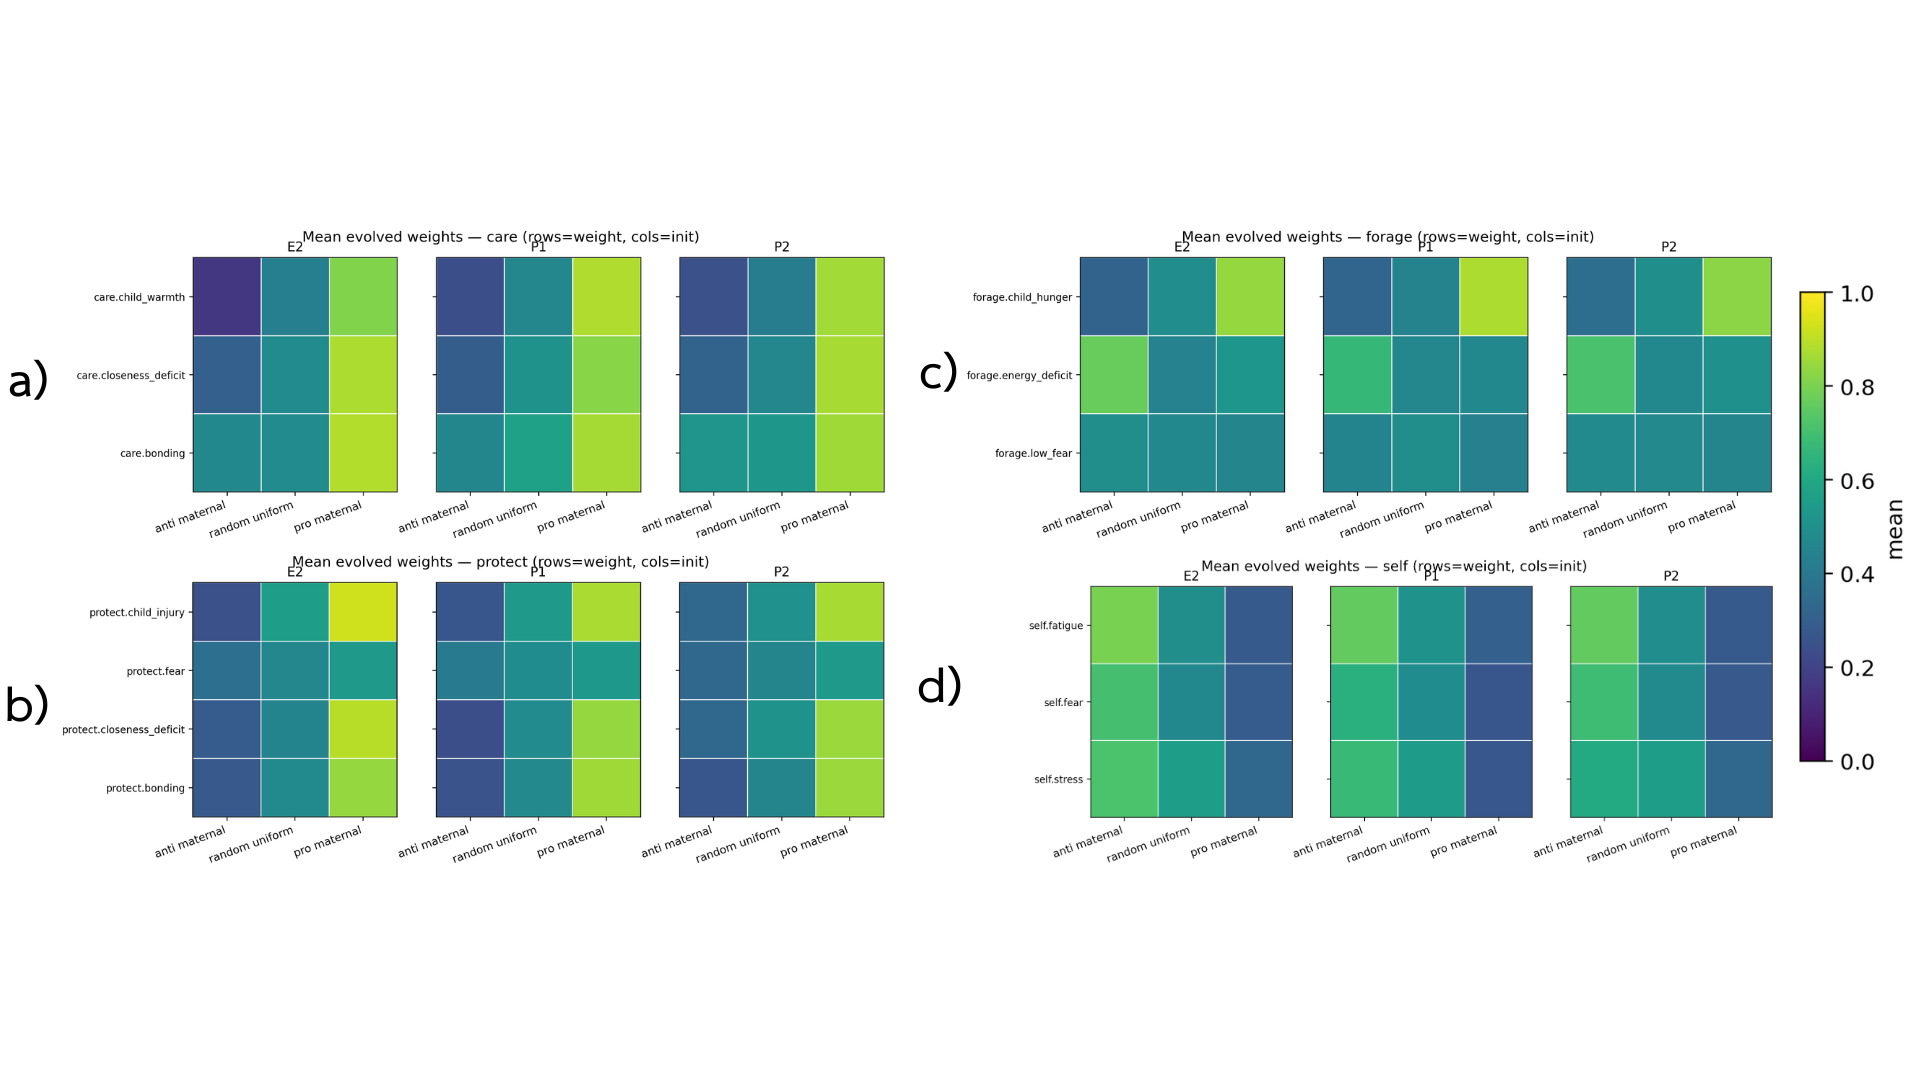
\includegraphics[width=\linewidth, trim={0 150 0 50}, clip]
    {plots/exp_3_weights.png}
    \caption{Selected motivation weights vs.\ generation ($3\times 3$: init $\times$ plasticity; mean $\pm$ IQR, 30 seeds).}
    \label{fig:exp3_weights}
\end{figure}

\begin{figure}[H]
    \centering
    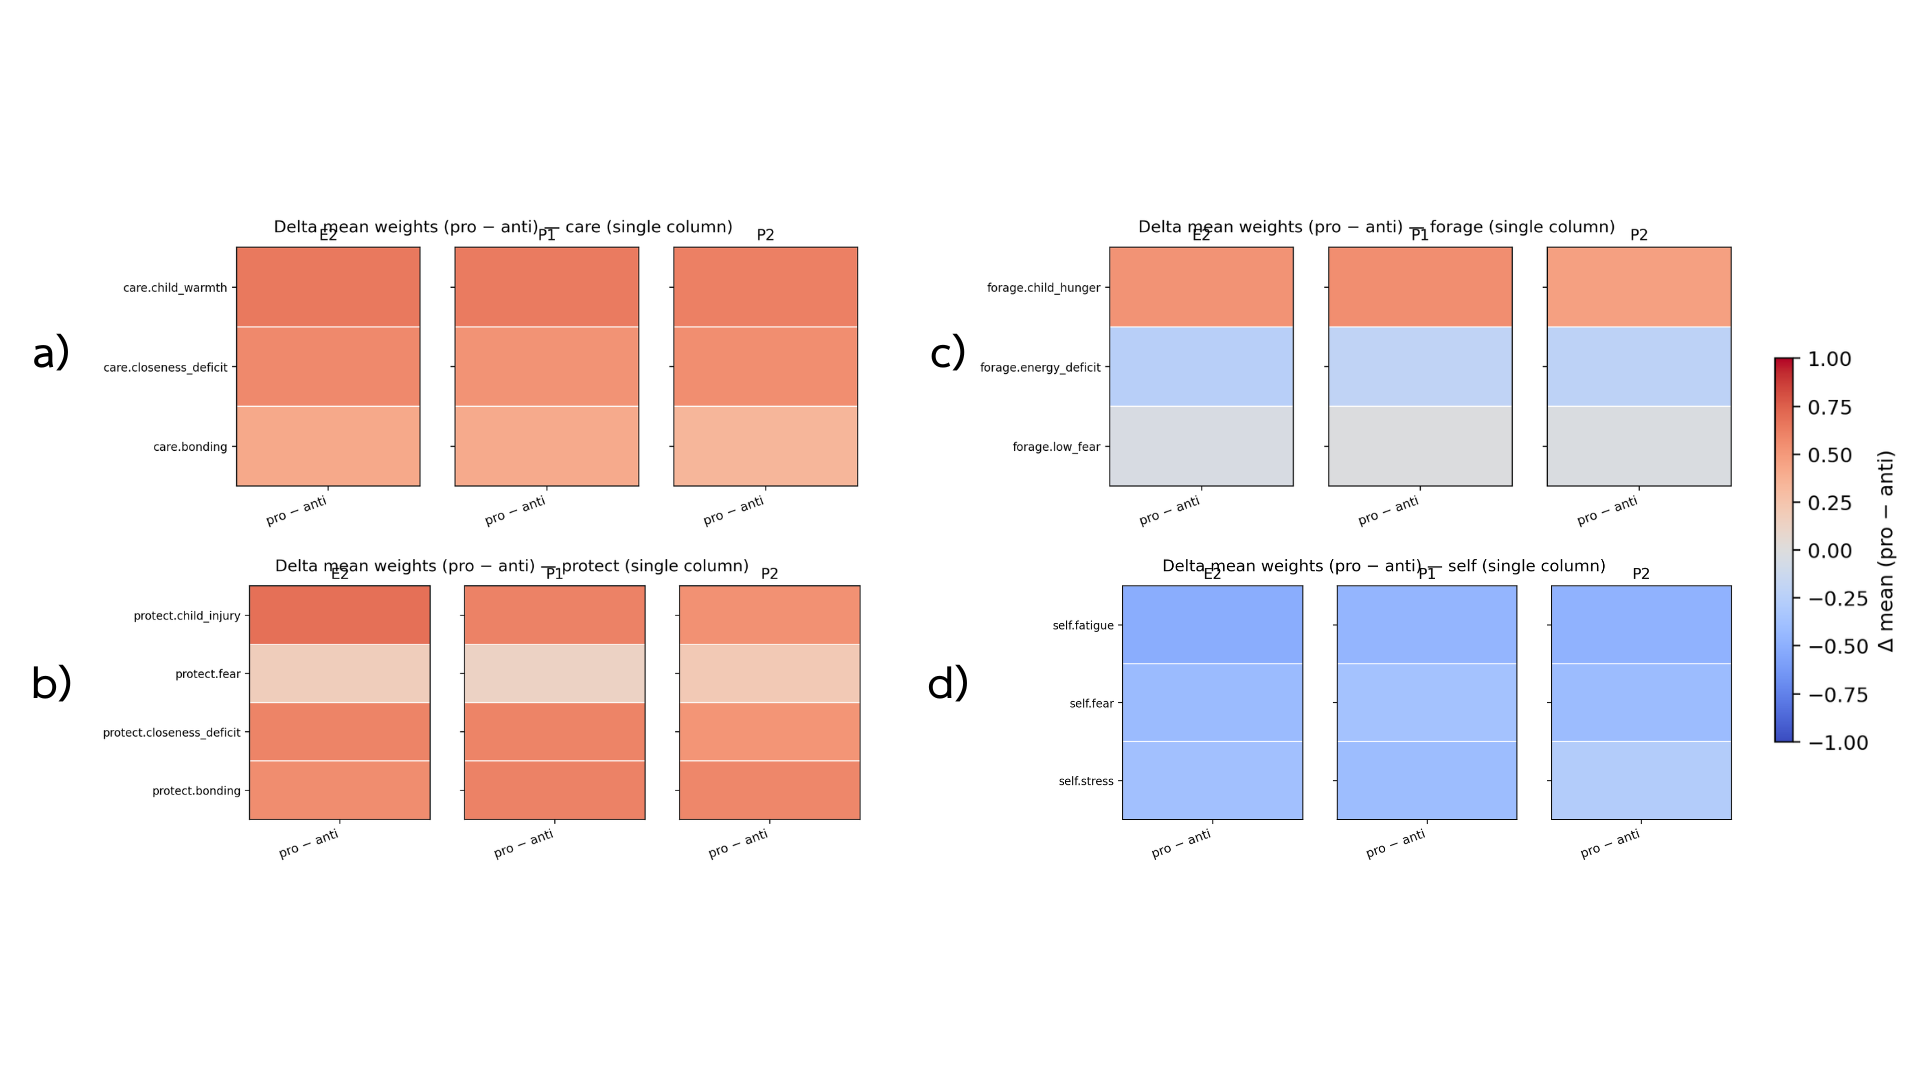
\includegraphics[width=\linewidth, trim={0 150 0 150}, clip]
    {plots/exp_3_diff_weights.png}
    \caption[Final weights (pro minus anti)]{Final weights: \texttt{pro\_maternal} minus \texttt{anti\_maternal} (mean over 30 seeds), per plasticity panel.}
    \label{fig:exp3_diff_weights}
\end{figure}

\subsection{Child survival and need-dependent behavior}
Figure~\ref{fig:exp3_child_ttd_bounds}: normalized child TTD rises from early to emergent stages for all inits/plasticities (vs.\ passive and strong-active reference bands)---evolution improves child survival.
Figure~\ref{fig:exp3_child_state_motivation}: conditional $P(\text{Forage}\mid\text{hungry})$, $P(\text{Care}\mid\text{cold})$, $P(\text{Protect}\mid\text{injured})$ increase toward need-appropriate switching; child physiology moves toward safer alive-tick ranges.

\begin{figure}[H]
    \centering
    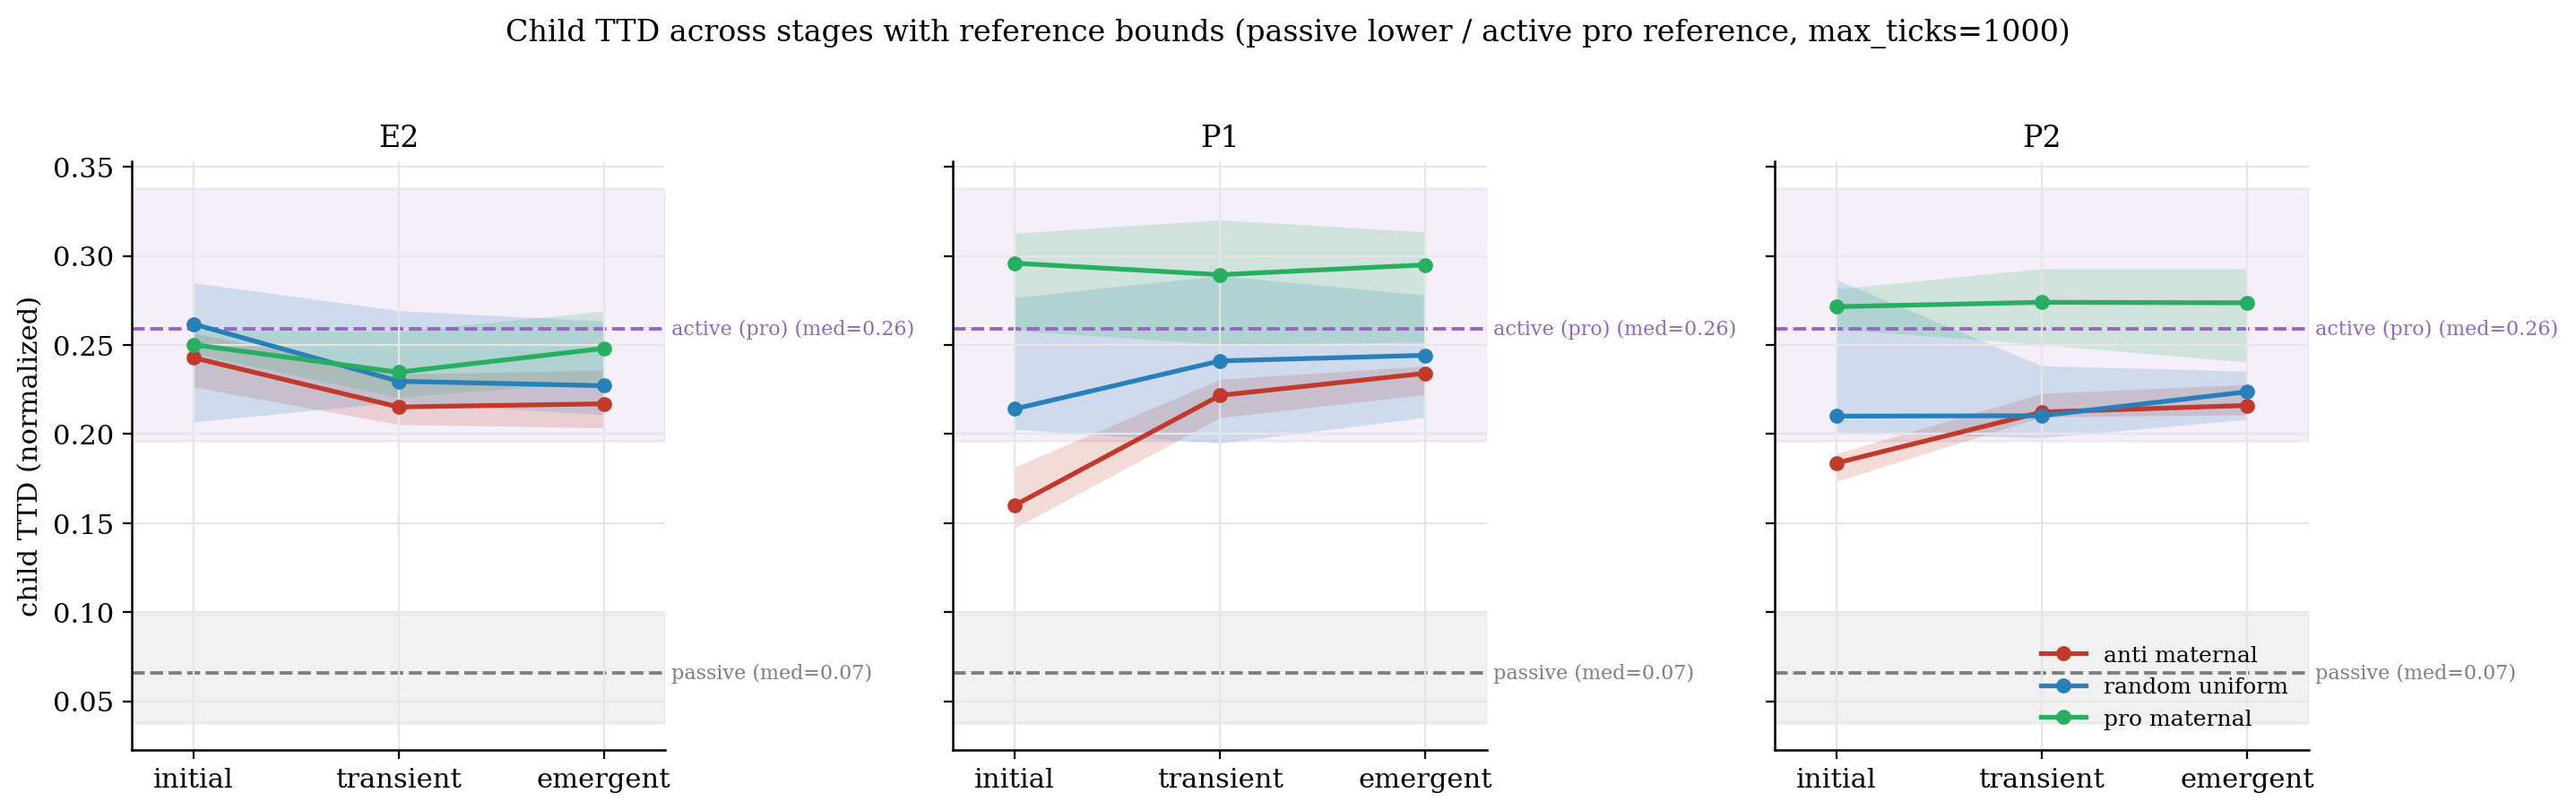
\includegraphics[width=\linewidth]{plots/exp_3_child_ttd_with_bounds_trajectory.png}
    \caption{Child TTD across evolutionary stages (E2/P1/P2 panels; init-colored medians with IQR across genomes).}
    \label{fig:exp3_child_ttd_bounds}
\end{figure}

\begin{figure}[H]
    \centering
    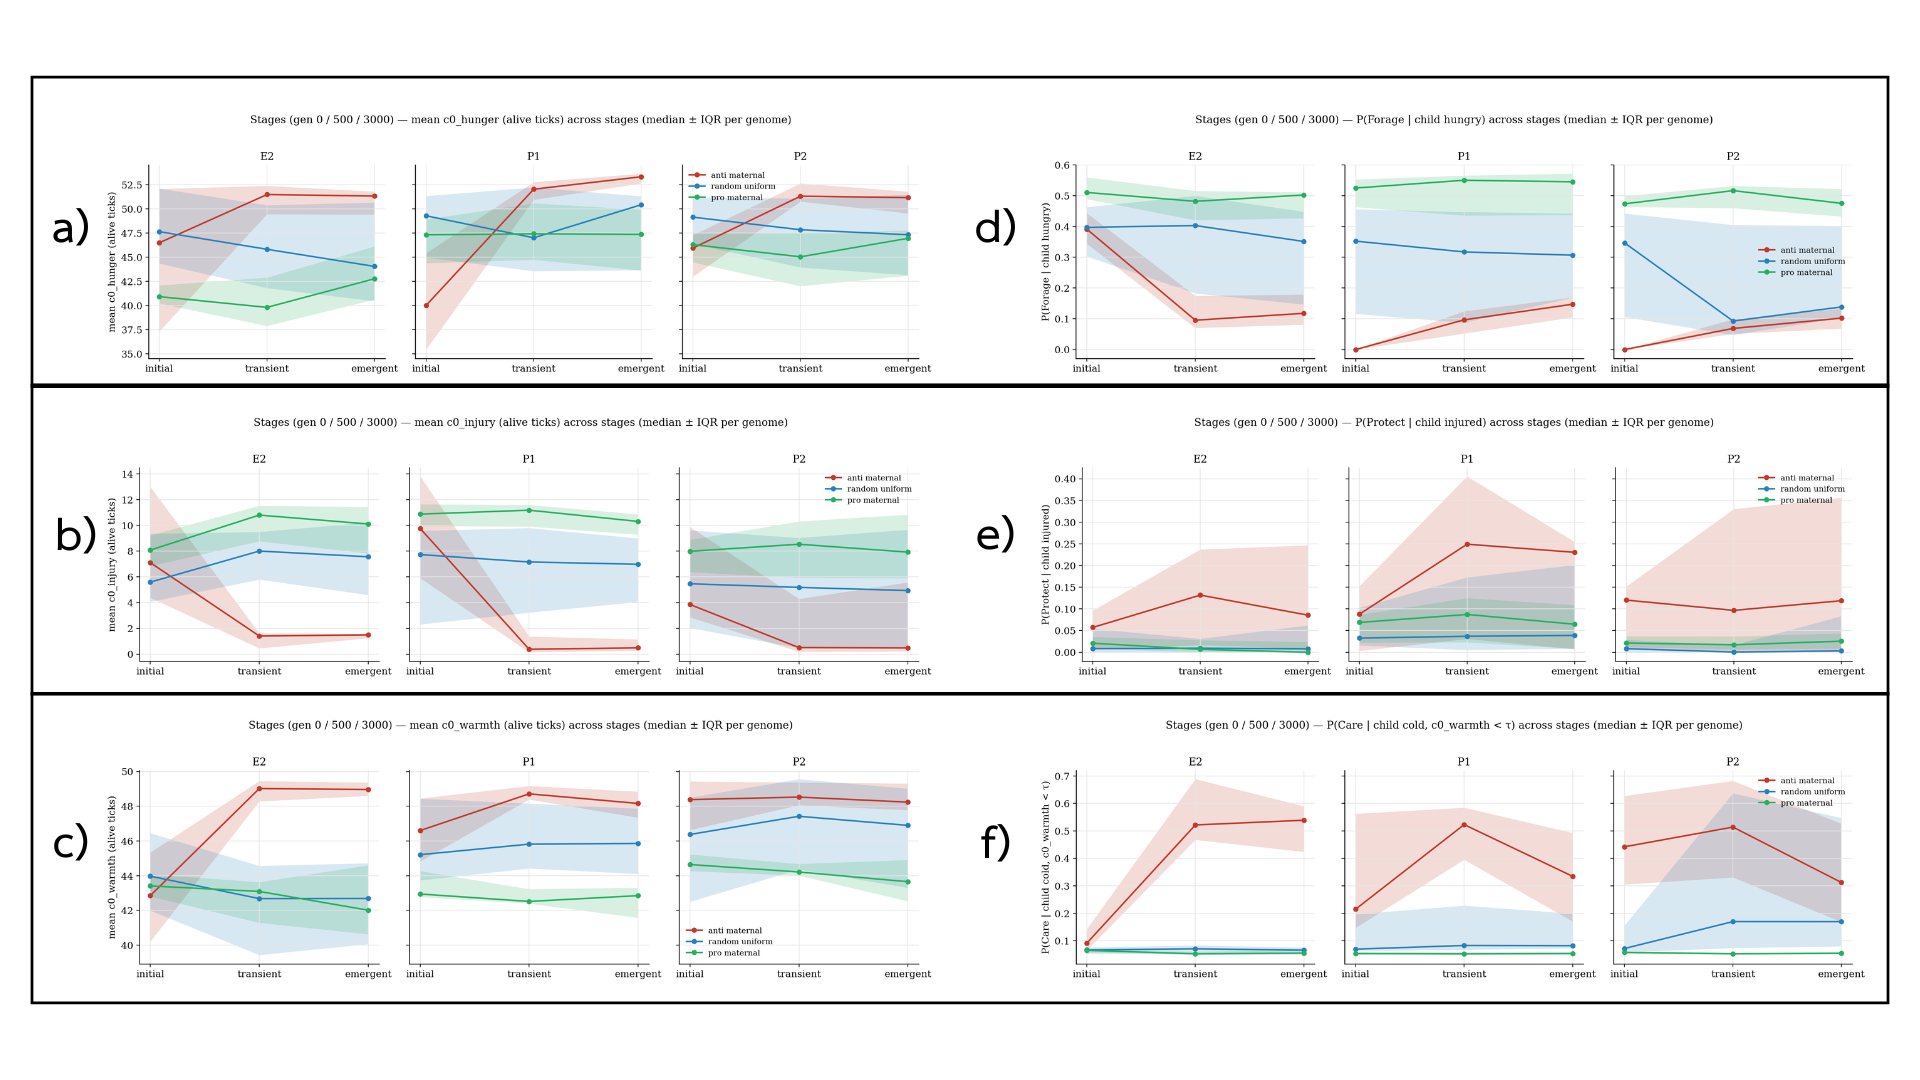
\includegraphics[width=\linewidth, trim={0 50 0 50}, clip]
    {plots/exp_3_child_state_motivation.png}
    \caption{Conditional motivation probabilities and mean child hunger/warmth/injury during emergence.}
    \label{fig:exp3_child_state_motivation}
\end{figure}

\subsection{Death causes on the seen world (normal, food interval 15)}
Figures~\ref{fig:exp3_death_cause}--\ref{fig:exp3_death_cause_merge} evaluate final genomes on the \emph{training-matched} ecology only (normal threats, medium food interval 15---not the full E4 grid).
Hunger is the dominant pooled failure for anti-maternal and random-uniform genomes; pro-maternal genomes show more balanced alive/cold/injury outcomes.

\begin{figure}[H]
    \centering
    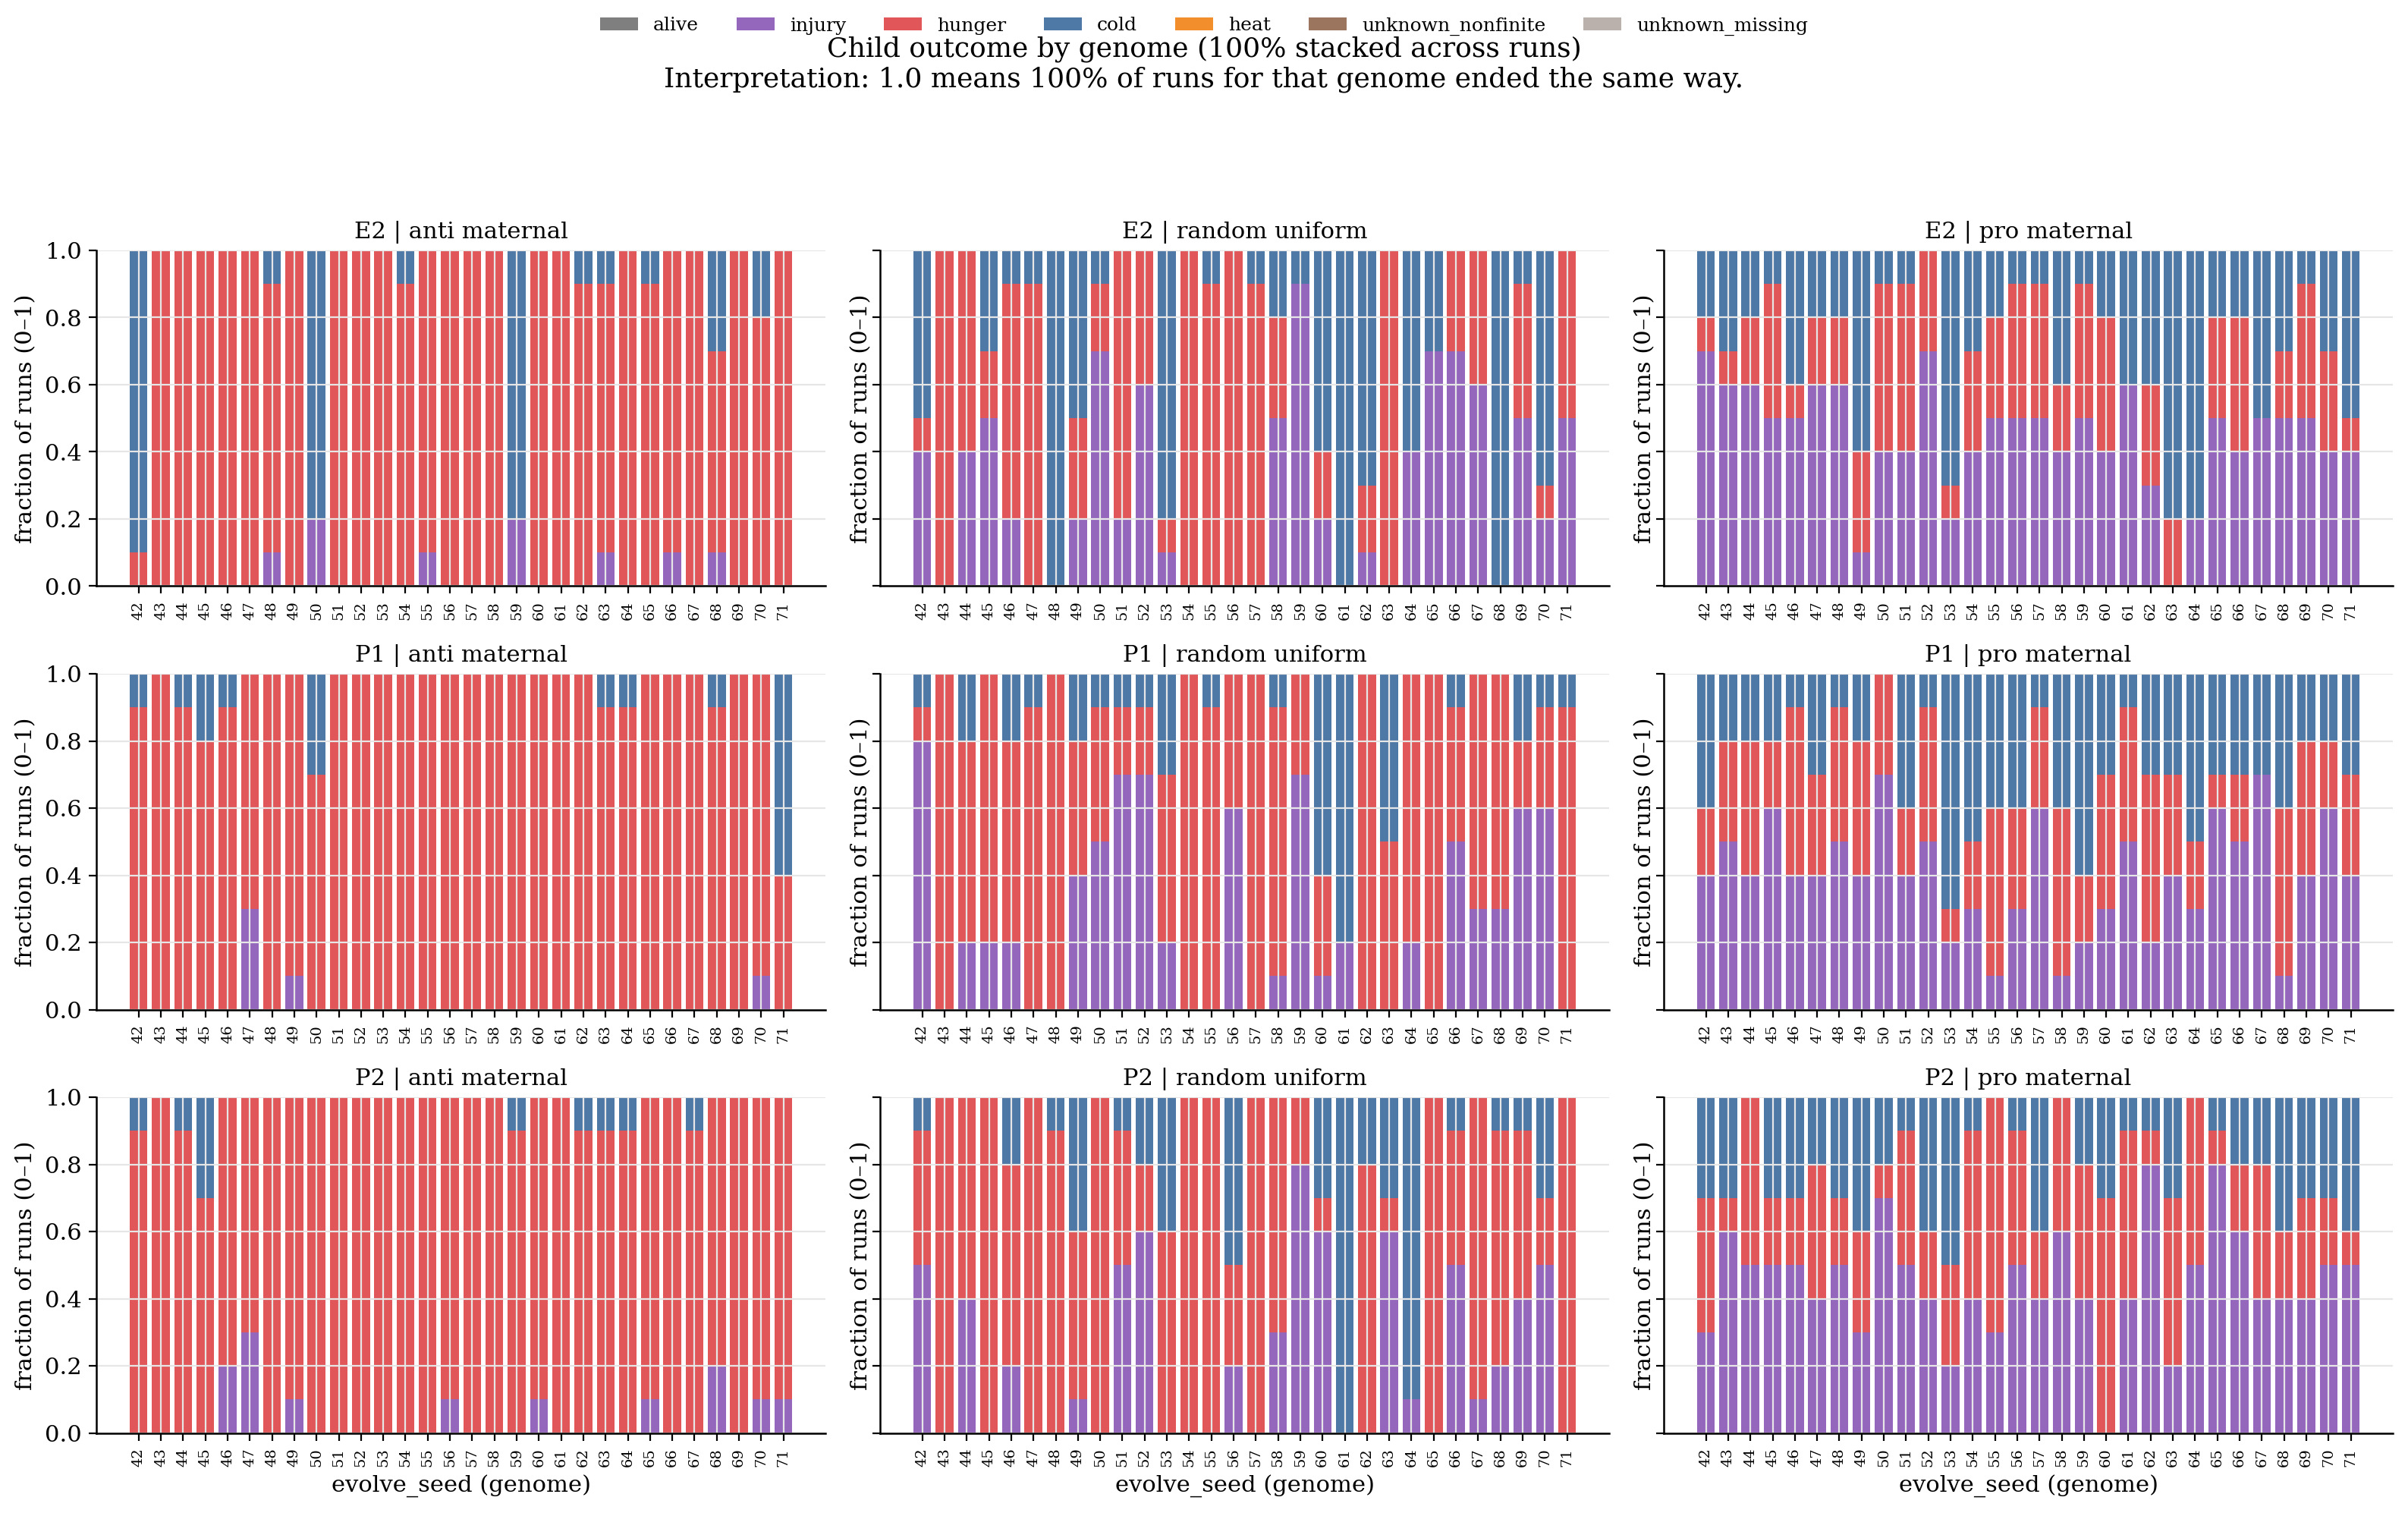
\includegraphics[width=\linewidth]{plots/exp_3_death_cause.png}
    \caption{Child outcomes on seen world (normal, food interval 15): per evolution seed (30 bars per panel; 10 rollouts each).}
    \label{fig:exp3_death_cause}
\end{figure}

\begin{figure}[H]
    \centering
    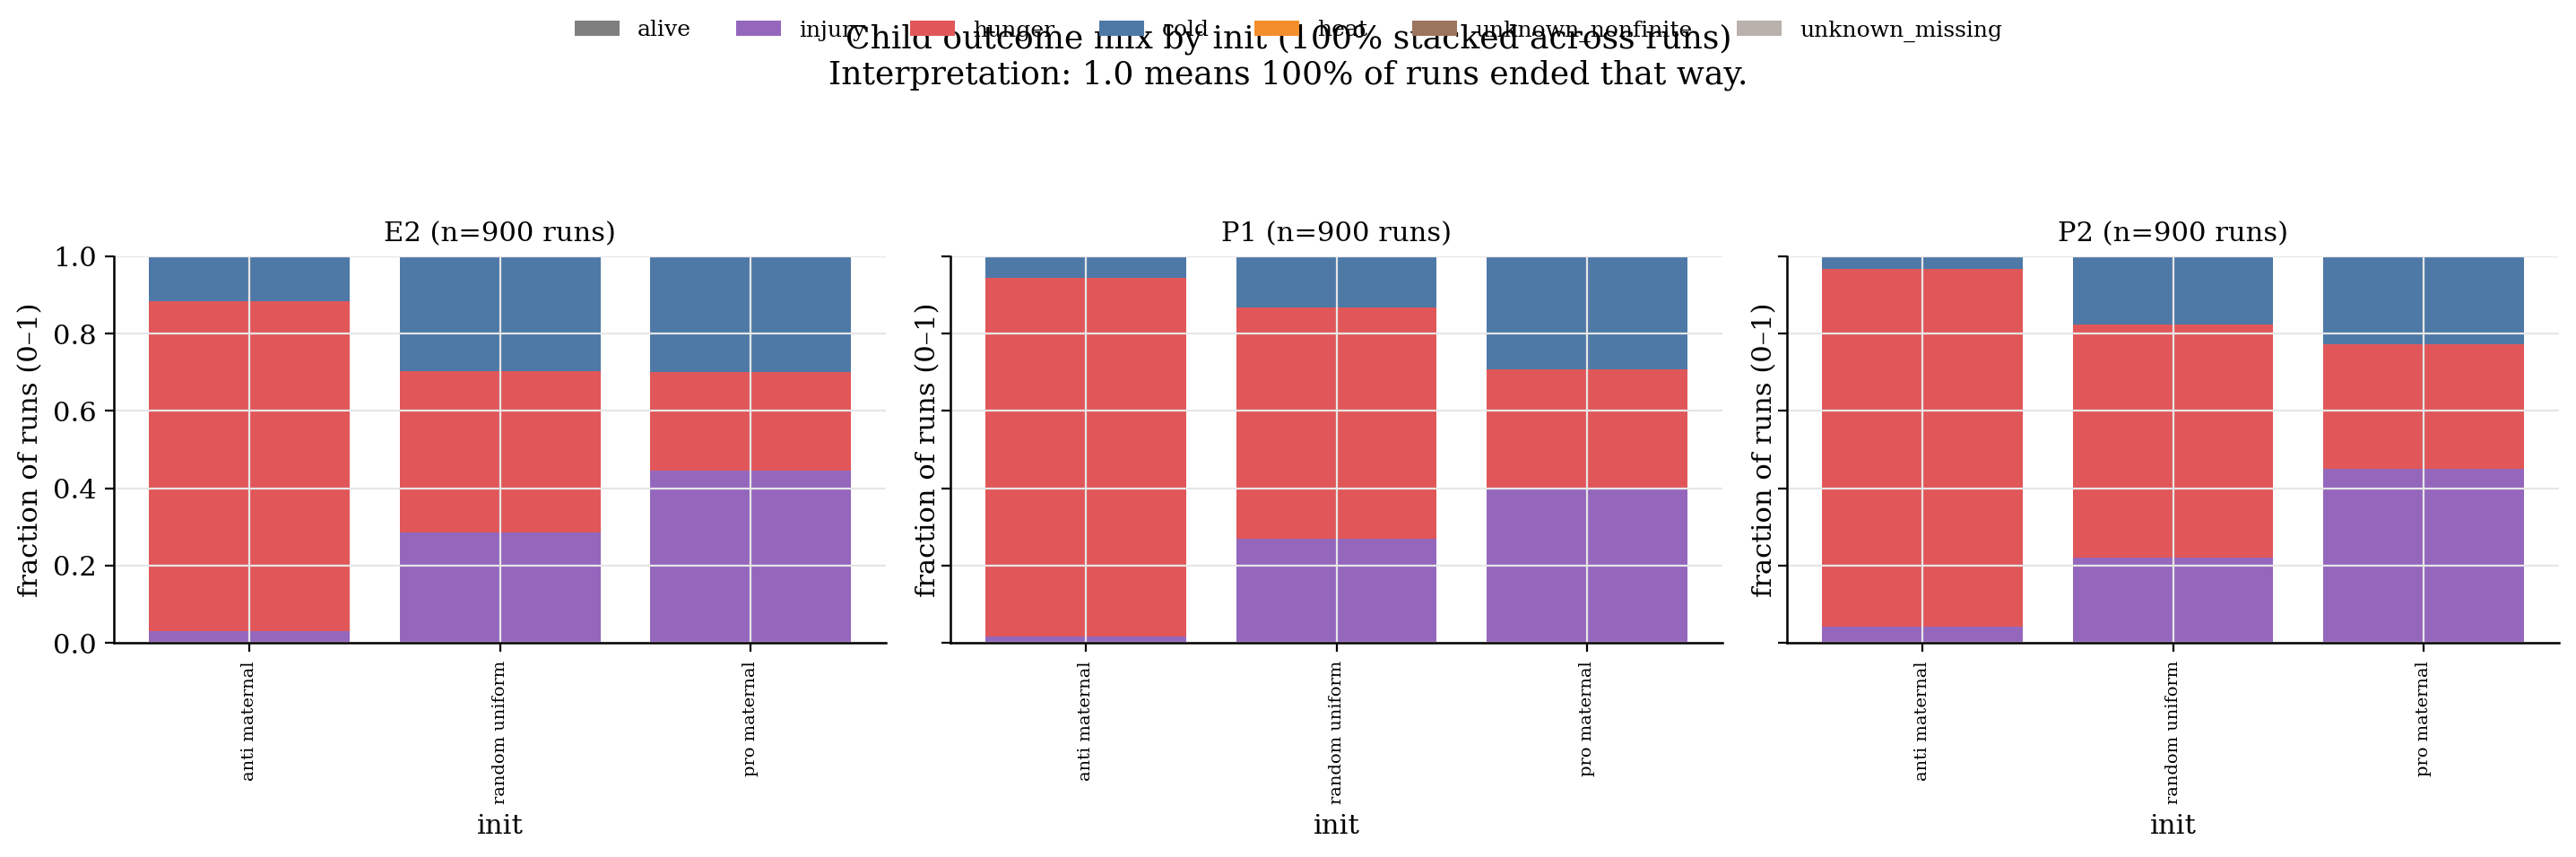
\includegraphics[width=\linewidth]{plots/exp_3_death_cause_merge.png}
    \caption{Same evaluation, pooled over seeds: three plasticity panels, one stacked bar per init.}
    \label{fig:exp3_death_cause_merge}
\end{figure}

\subsection{Takeaway (Experiment 3)}
Anti-maternal priors require the largest genome displacement; pro-maternal the smallest; all inits improve child TTD and conditional care, but hunger failures remain more common for anti-maternal genomes on the training ecology.

% =============================================================================
\section{Experiment 4: Generalization to unseen environments (E4)}
\subsection{Unseen condition grid}
Final genomes from emergence are evaluated on nine cells: world $\{easy, normal, hard\}$ $\times$ food spawn interval $\{5, 15, 25\}$, where \textbf{5 = abundant}, \textbf{15 = medium} (training), \textbf{25 = scarce}.
Ten rollouts per genome per cell; 30 seeds per (plasticity, init) $\Rightarrow$ 300 episodes per tile in death-cause figures.

\subsection{Transfer performance}
Figure~\ref{fig:exp4_unseen}: performance is best on \textbf{easy} worlds and at \textbf{food~5} (abundant); worst on \textbf{hard} worlds and at \textbf{food~25} (scarce).
Pro-maternal curves often sit above anti-maternal on mild cells; gaps shrink on the harshest corners.

\begin{figure}[H]
    \centering
    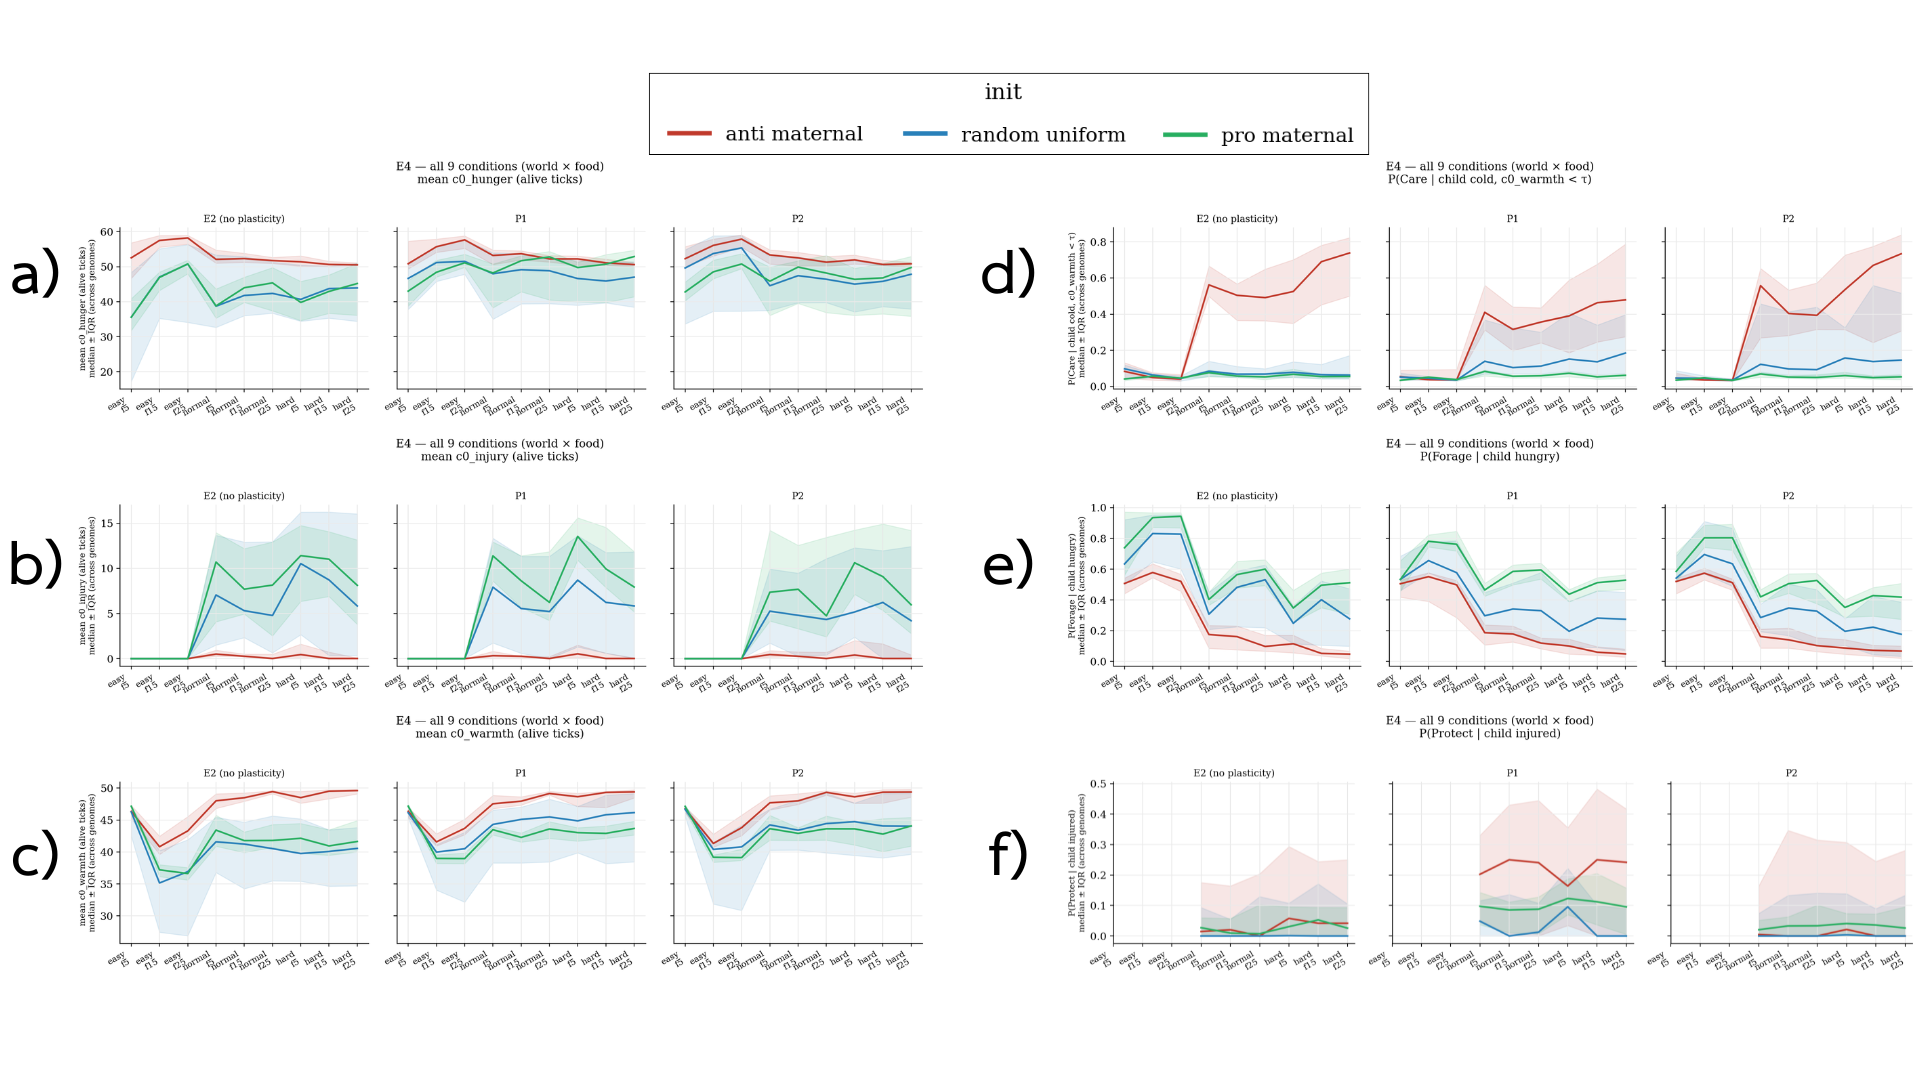
\includegraphics[width=\linewidth, trim={0 50 0 50}, clip]
    {plots/exp_4_unseen.png}
    \caption{E4 transfer on the $3\times 3$ grid (world $\times$ food interval 5/15/25; 5 = abundant, 25 = scarce). Columns: E2/P1/P2; line color: init.}
    \label{fig:exp4_unseen}
\end{figure}

\subsection{Child and mother TTD on the grid}
Figures~\ref{fig:exp4_child_TTD} and~\ref{fig:exp4_mother_TTD}: child TTD falls most on hard worlds and at food~25 (scarce); comparing panels separates child-only failure from joint mother--child mortality.

\begin{figure}[H]
    \centering
    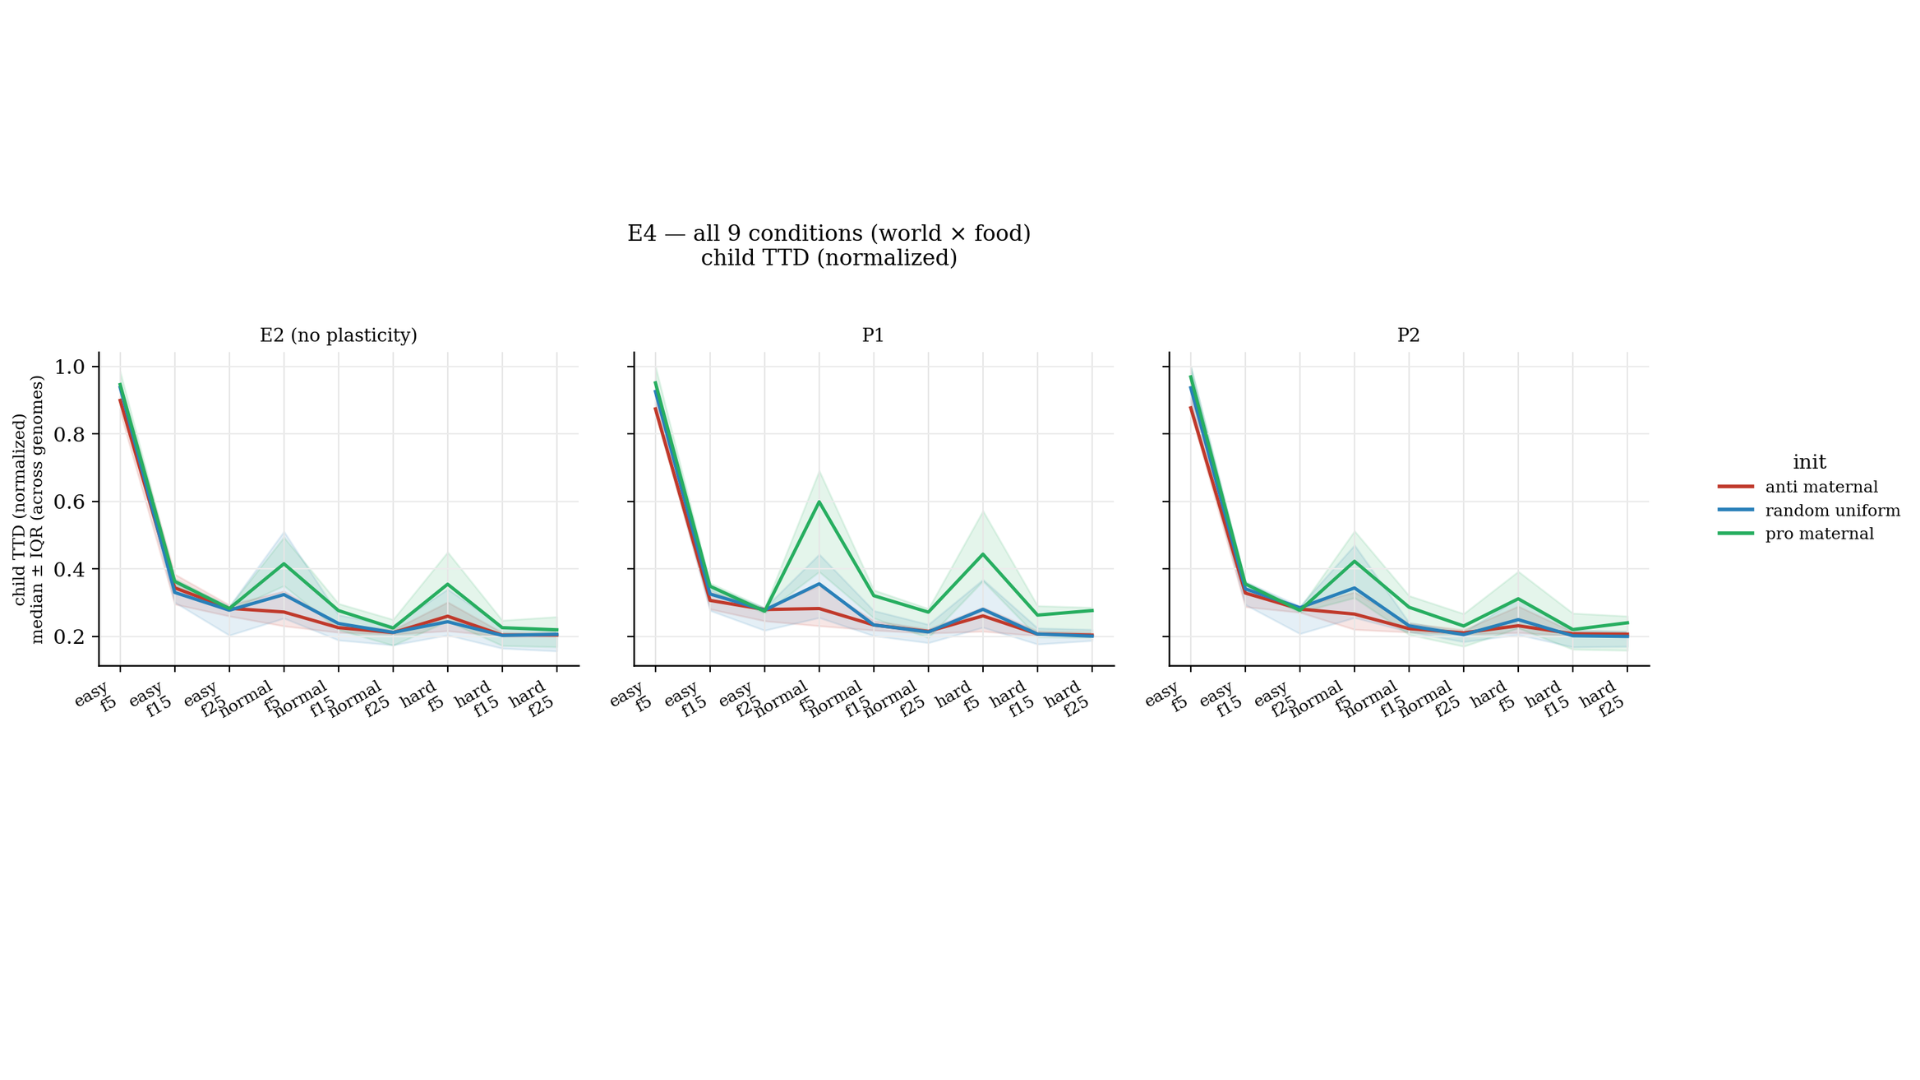
\includegraphics[width=\linewidth, trim={0 250 0 150}, clip]
    {plots/exp_4_child_TTD.png}
    \caption{Normalized child TTD on nine E4 cells (median $\pm$ IQR over 30 genomes).}
    \label{fig:exp4_child_TTD}
\end{figure}

\begin{figure}[H]
    \centering
    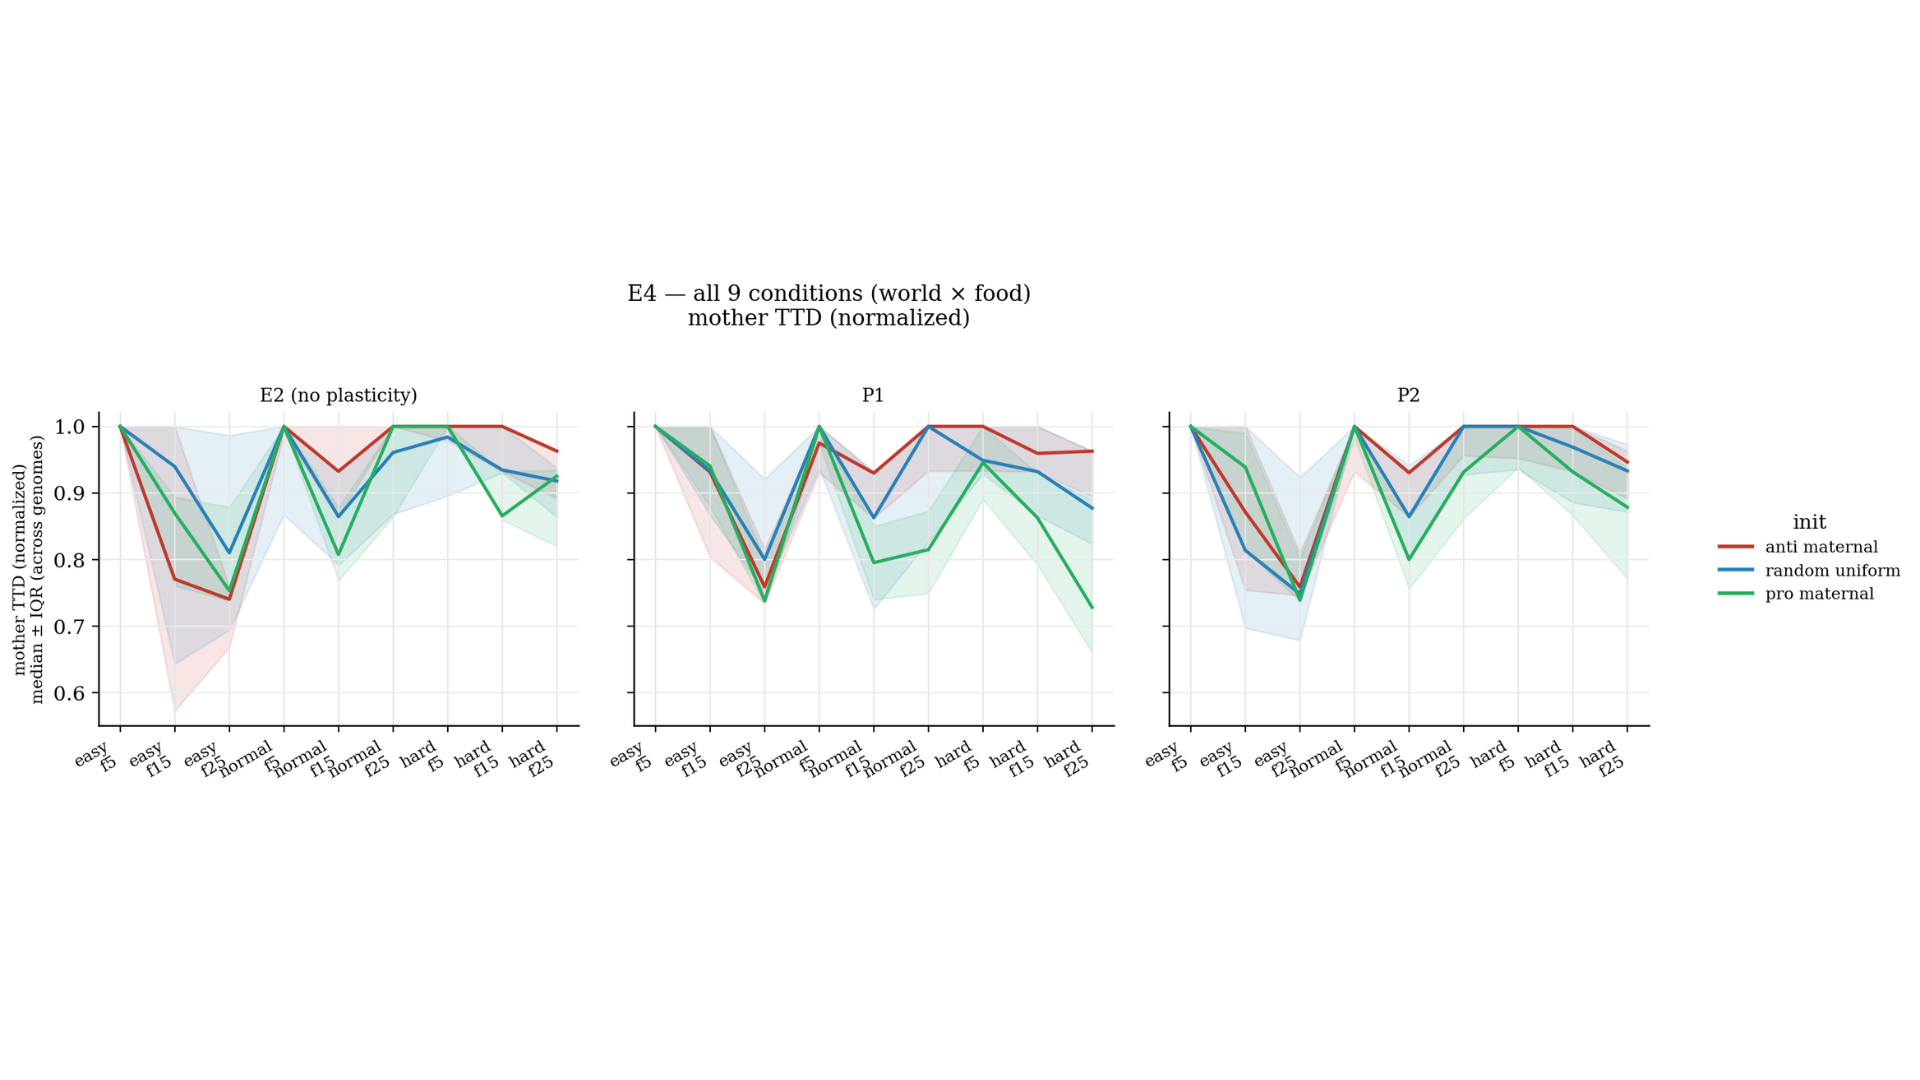
\includegraphics[width=\linewidth, trim={0 250 0 150}, clip]
    {plots/exp_4_mother_TTD.png}
    \caption{Normalized mother TTD on nine E4 cells (same layout as child panel).}
    \label{fig:exp4_mother_TTD}
\end{figure}

\subsection{Death causes per cell and pooled}
Figure~\ref{fig:exp4_dominant_cause}: on easy rows and at food~5, \textbf{alive} (A) is often plurality; on normal/hard rows and at food~25, \textbf{hunger} (hun) dominates many anti-maternal tiles.
Figures~\ref{fig:exp4_death_seeds}--\ref{fig:exp4_death_merge}: all nine cells pooled ($90$ rollouts per seed).

\begin{figure}[H]
    \centering
    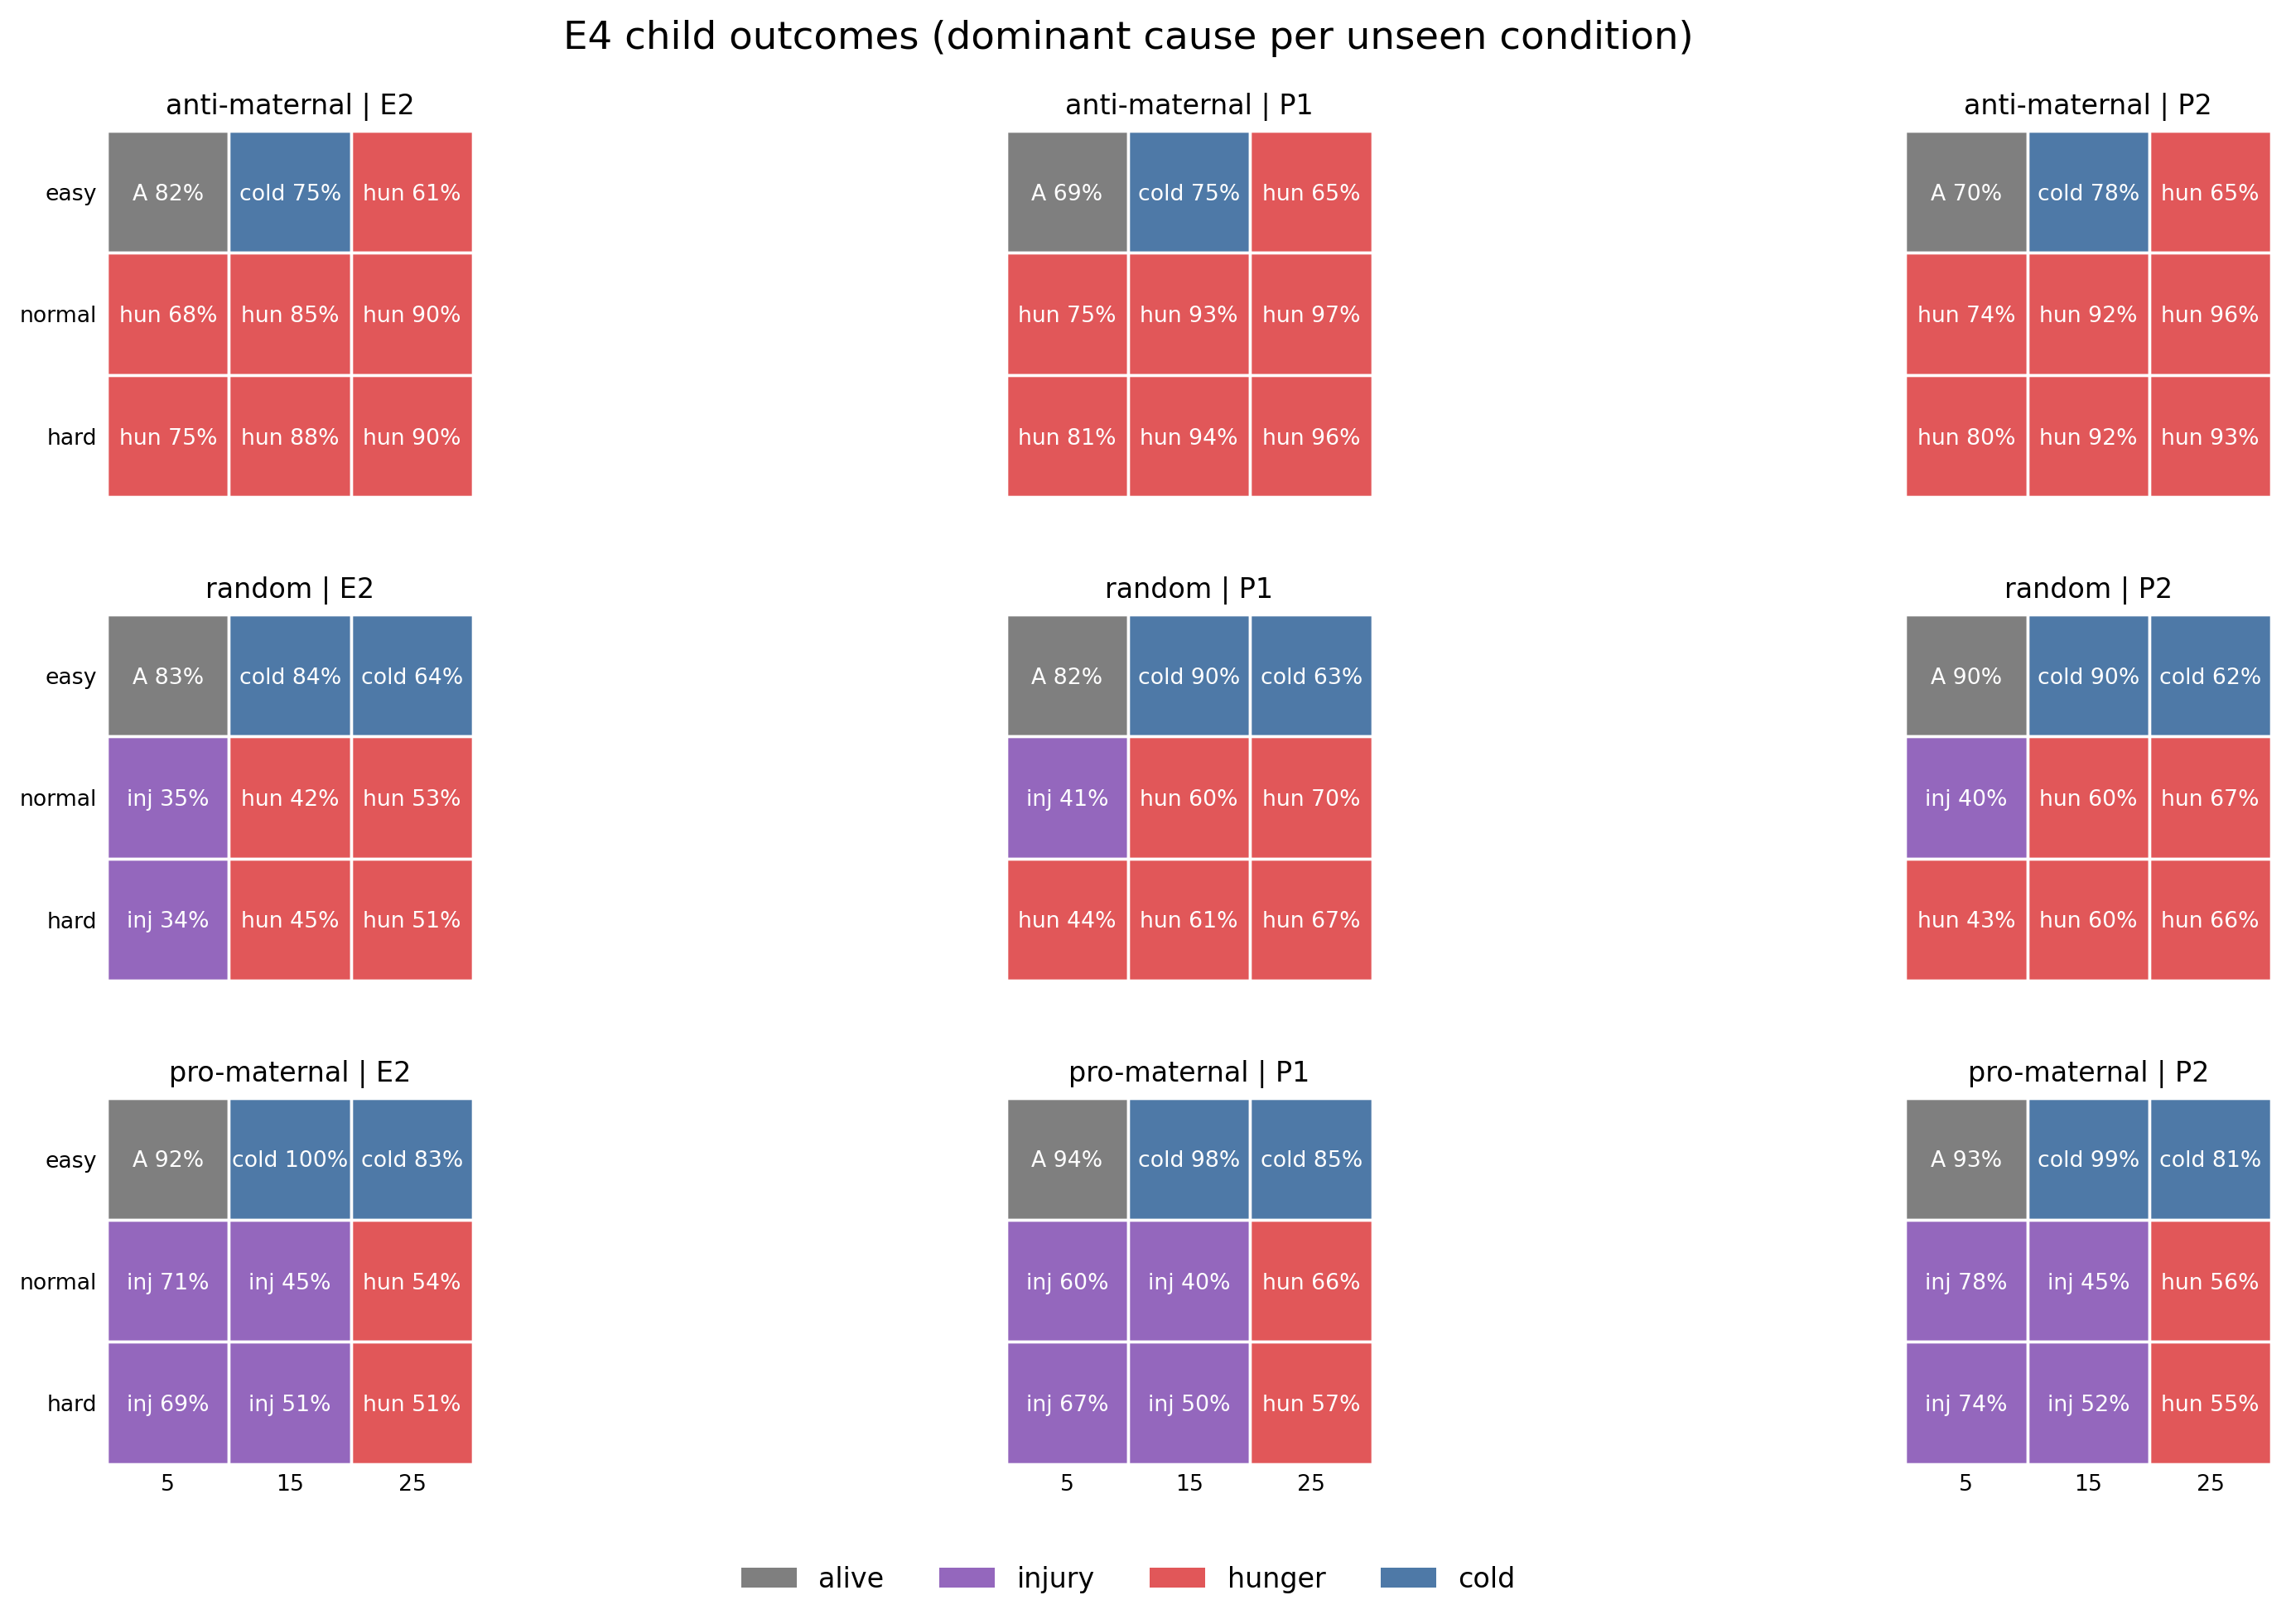
\includegraphics[width=\linewidth]{plots/exp_4_dominant_cause.png}
    \caption{Dominant child outcome per E4 cell (A/hun/cold/inj; \% over 300 rollouts). Insets: world (rows) $\times$ food 5/15/25 (cols; 5 abundant, 25 scarce).}
    \label{fig:exp4_dominant_cause}
\end{figure}

\begin{figure}[H]
    \centering
    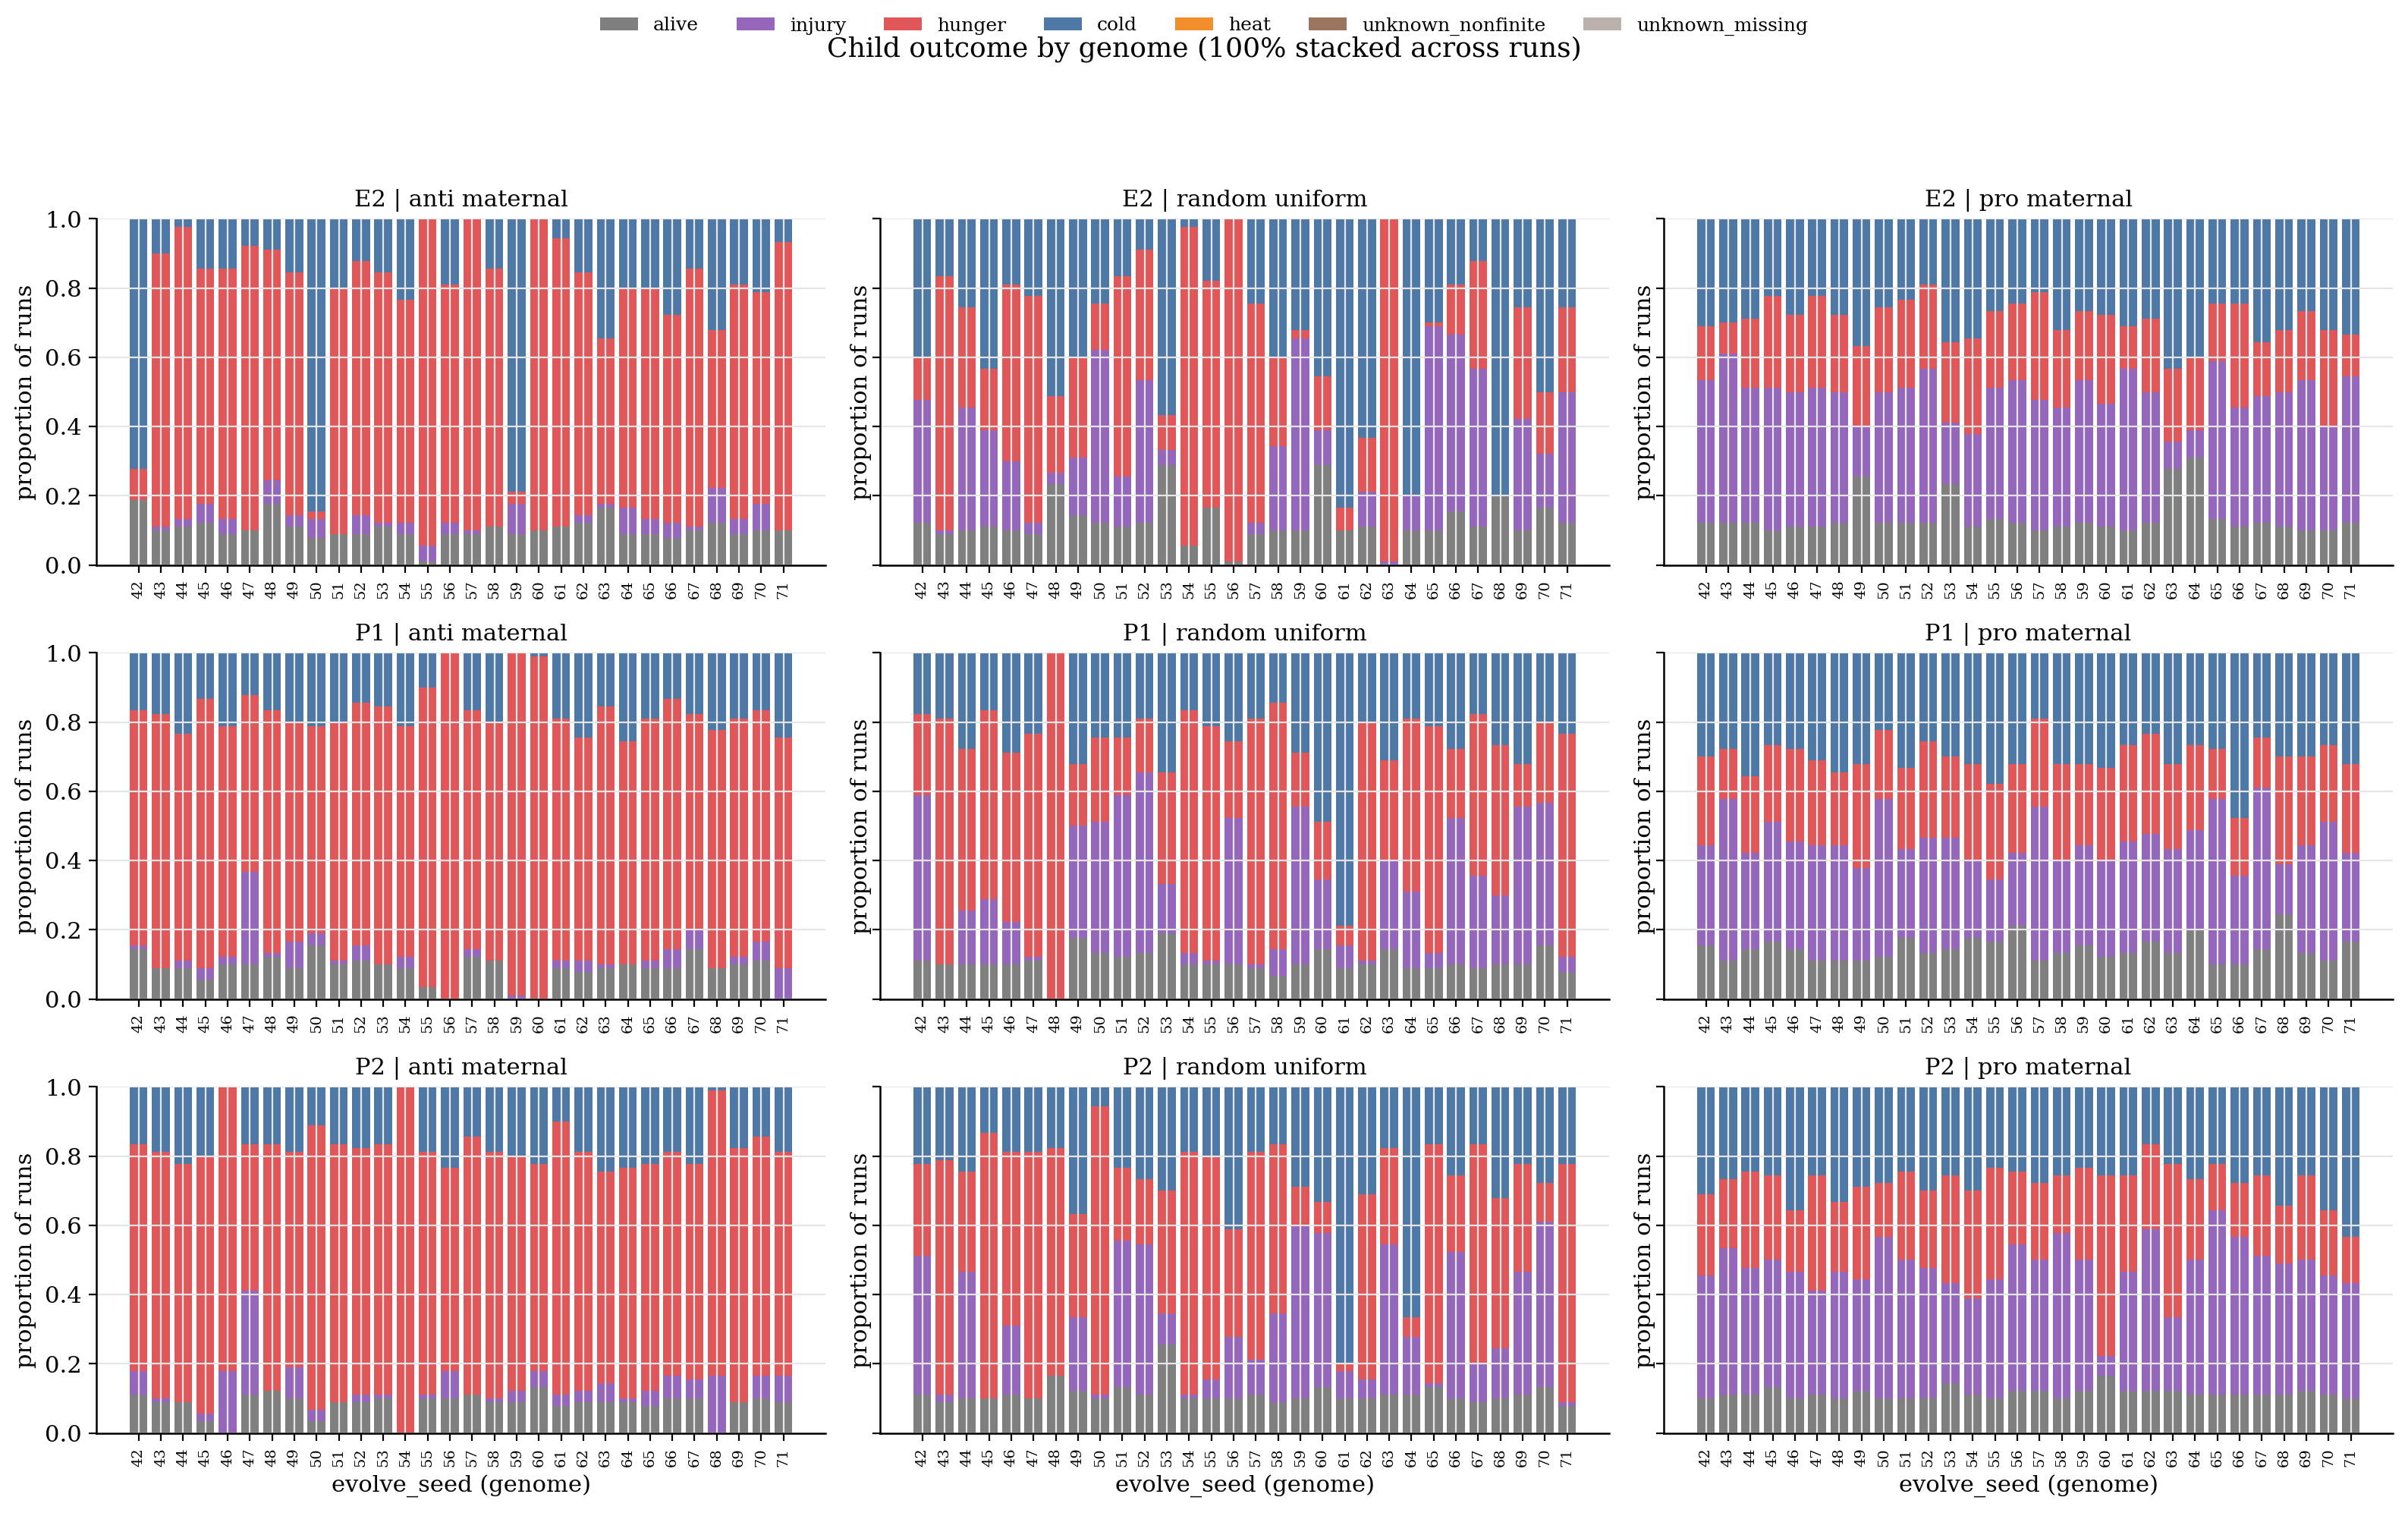
\includegraphics[width=\linewidth]{plots/exp_4_death_seeds.png}
    \caption{Outcomes pooled over all nine E4 cells, per evolution seed ($9\times 10$ rollouts per bar).}
    \label{fig:exp4_death_seeds}
\end{figure}

\begin{figure}[H]
    \centering
    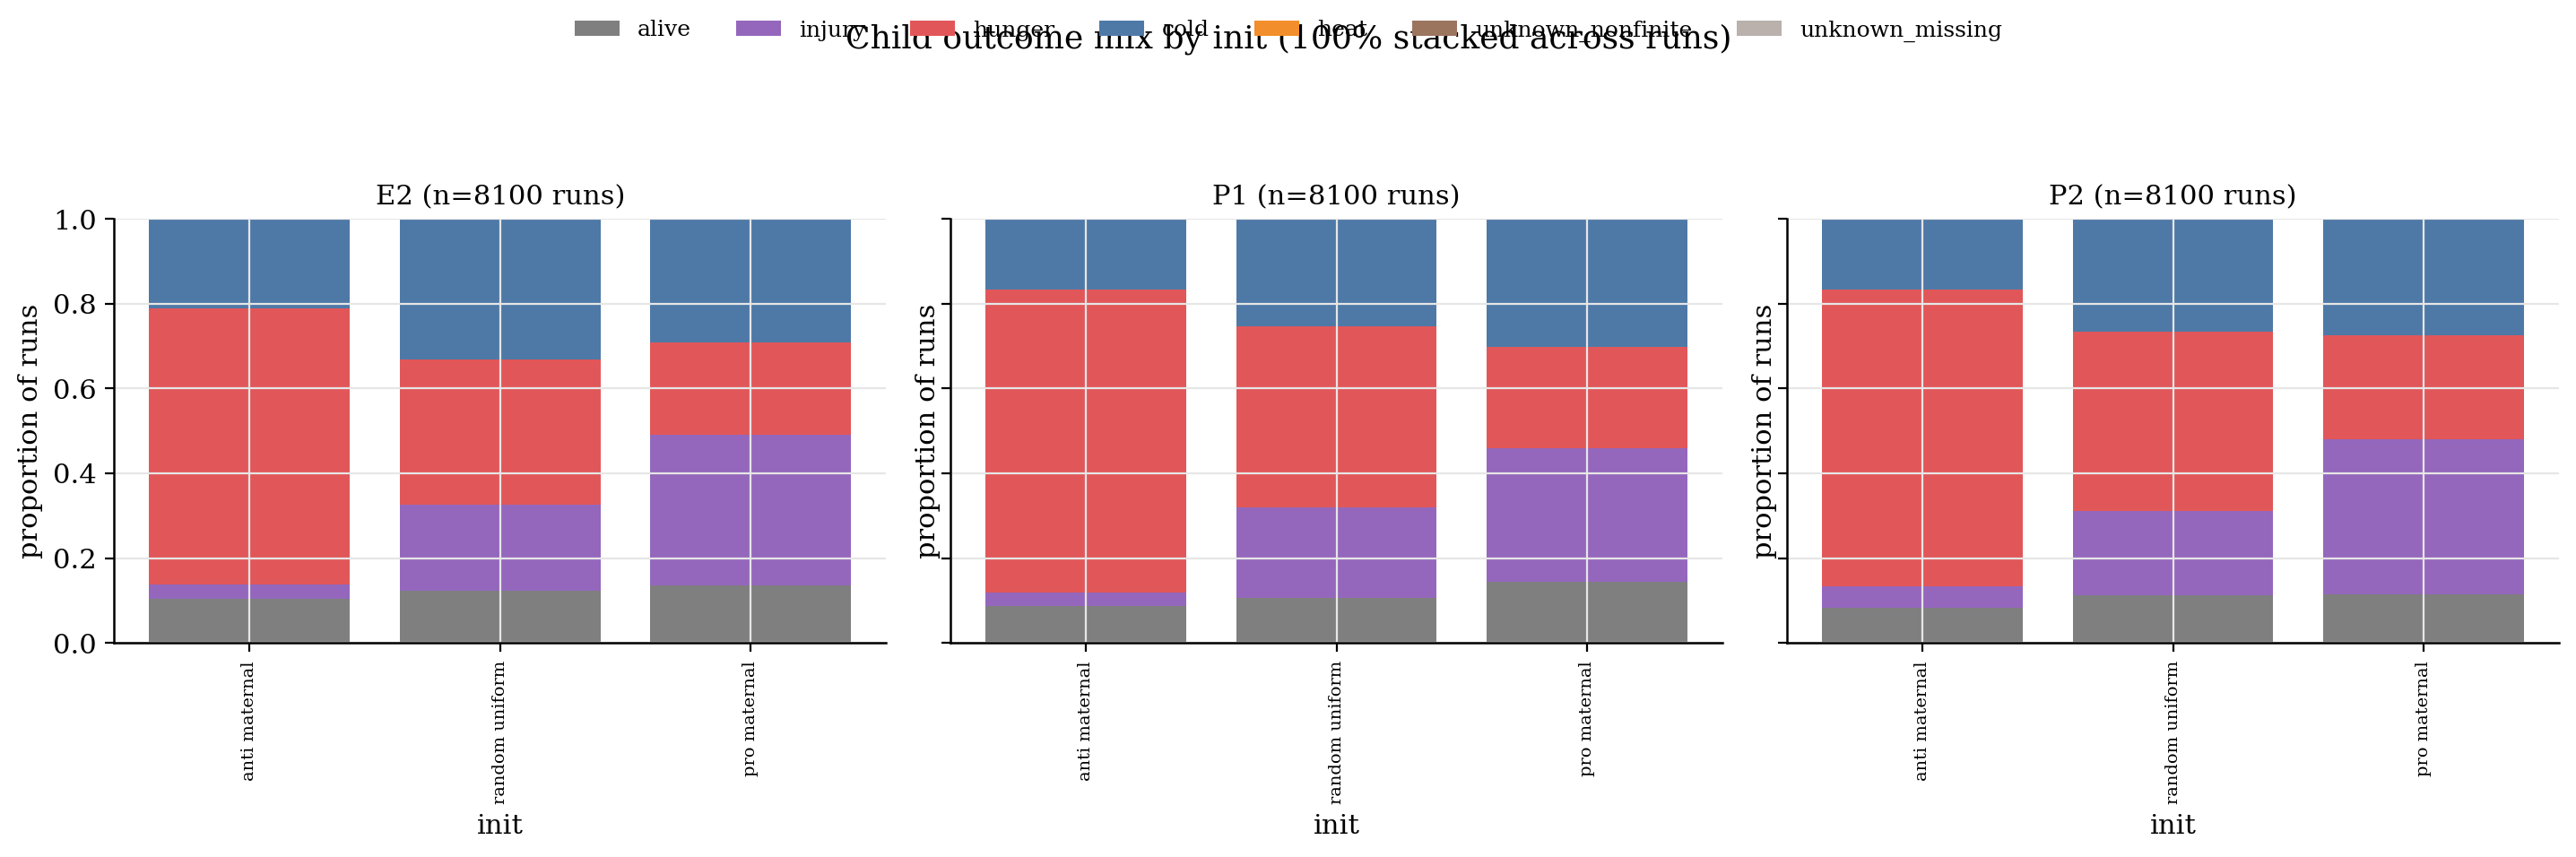
\includegraphics[width=\linewidth]{plots/exp_4_death_merge.png}
    \caption{Same nine-cell pool, summarized by (plasticity, init).}
    \label{fig:exp4_death_merge}
\end{figure}

\subsection{Takeaway (Experiment 4)}
Transfer is graded: easy worlds and abundant food (interval~5) preserve child survival; hard worlds and scarce food (interval~25) produce hunger-dominated failure. Agents generalize to milder transfer cells better than to the scarcest-food, highest-threat corners.

% =============================================================================
\section{Chapter summary}

\begin{table}[H]
  \centering
  \caption{Summary of experimental questions and main outcomes.}
  \label{tab:exp_summary}
  \small
  \begin{tabular}{p{0.14\linewidth}p{0.36\linewidth}p{0.42\linewidth}}
    \toprule
    \textbf{Exp} & \textbf{Question} & \textbf{Main outcome} \\
    \midrule
    1 & Maternal behavior in training world? &
    Survival and states differ by condition; effective policies coordinate motivations and physiology. \\
    2 & Plasticity / Baldwin? &
    P1/P2 outperform E2 in fitness rise; large early plastic updates. \\
    3 & Init priors shape evolution? &
    Anti drifts most, pro least; care/TTD improve for all; hunger bias remains for anti on seen world. \\
    4 & Generalization (E4)? &
  Good on easy + abundant food (5); poor on hard + scarce food (25); hunger dominates harsh cells. \\
    \bottomrule
  \end{tabular}
\end{table}

Overall, need-dependent maternal policies can evolve from anti-maternal starts, plasticity speeds search, and transfer fails predictably when threat pressure and food scarcity (interval~25) exceed the training regime (normal world, interval~15).
